% This file was converted to LaTeX by Writer2LaTeX ver. 1.0.2
% see http://writer2latex.sourceforge.net for more info
\documentclass[a5paper,headsepline,titlepage,11pt,nnormalheadings,DIVcalc,openany]{scrbook}
\usepackage[a5paper,backref]{hyperref}
\usepackage[papersize={165mm,215mm},twoside,bindingoffset=0.5cm,hmargin={2cm,2cm},
				vmargin={2cm,2cm},footskip=1.1cm,driver=dvipdfm]{geometry}
\usepackage[latin1]{inputenc}
\usepackage[T1]{fontenc}
\usepackage[bahasa]{babel}
\usepackage{microtype}
\usepackage{palatino}
\usepackage{amssymb,amsfonts,textcomp}
\usepackage{array}
\usepackage{longtable}
\usepackage{hhline}
\usepackage[pdftex]{graphicx}
\usepackage{graphvizzz}
\usepackage{multirow}
\usepackage{enumitem}
\usepackage{marvosym}
\usepackage{pstricks}
\usepackage{floatflt}
\usepackage{fancyhdr}

\makeatletter
\newcommand\arraybslash{\let\\\@arraycr}
\makeatother
\setlength\tabcolsep{1mm}
\renewcommand\arraystretch{1.3}
\title{Lingkungan St. Theresia Kanak-kanak Yesus}

\newcounter{nourut}
\newcommand{\nexturut}{%
\stepcounter{nourut}
\arabic{nourut}}
\renewcommand{\footrulewidth}{0.0pt}
\renewcommand{\headrulewidth}{0.0pt}
\lhead[\fancyplain{}{ \thepage}]%
      {\fancyplain{}{}}
\rhead[\fancyplain{}{}]%
      {\fancyplain{}{\thepage}}
\cfoot{}
\pagestyle{fancy}

\hyphenation{Bu-di-man di-so-si-al-i-sa-si-kan pe-ra-sa-nya di-a-jar-kan ber-ke-nan Tu-han}



\begin{document}
\thispagestyle{empty}
\DeclareFixedFont{\PT}{T1}{ppl}{b}{}{0.7in}
\DeclareFixedFont{\PTit}{T1}{ppl}{b}{it}{0.7in}
\DeclareFixedFont{\PTsmall}{T1}{ppl}{b}{it}{0.25in}
\DeclareFixedFont{\PTsmaller}{T1}{ppl}{b}{it}{0.175in}
\DeclareFixedFont{\PTsmallest}{T1}{ppl}{b}{it}{0.15in}

\begin{pspicture}(14cm,1cm)
\rput[cb](5.6cm,1.25cm){\PTsmall {Informasi Lingkungan}}
\rput[cb](5.6cm,0cm){\PTit {St. Theresia}}
\end{pspicture}%

\vspace{0.5cm}
\begin{center}
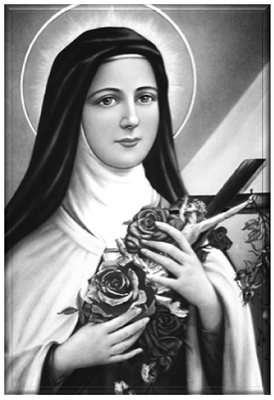
\includegraphics[scale=5]{theresia-bw.png}
\end{center}

\begin{pspicture}(14cm,1.5cm)
\rput[cb](5.6cm,1.5cm){\PTsmall {Wilayah Don Bosco, Stasi Maguwo}}
\rput[cb](5.6cm,0.75cm){\PTsmall {Paroki Marganingsih Kalasan}}
\rput[cb](5.6cm,0cm){\PTsmall {2015}}
\end{pspicture}%

\tableofcontents
\setlength{\parindent}{30pt}
\chapter{Sejarah Lingkungan}

\section{Lingkungan St. Theresia Kanak-kanak Yesus}
\begin{floatingfigure}[l]{2cm}
\begin{center}
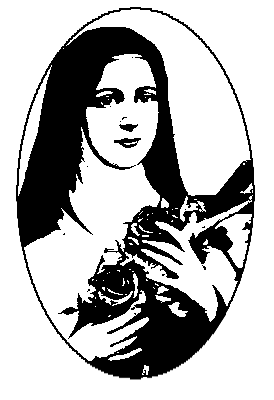
\includegraphics[scale=1]{theresia-logo.png}
\end{center}
\end{floatingfigure}
Lingkungan Santa Theresia Kanak-kanak Yesus adalah lingkungan baru di Stasi Bunda Maria Maguwo. Lingkungan ini merupakan hasil pemekaran dari lingkungan St. Petrus yang dirasa sudah terlalu banyak anggotanya. Lingkungan St. Petrus dimekarkan menjadi lingkungan St. Petrus, lingkungan St. Monika, dan lingkungan St. Theresia.

Pada akhir tahun 2013 yaitu pada bulan September, semua lingkungan di Stasi Maguwo 
diharapkan melakukan pemilihan pengurus baru. Sesuai dengan mekanisme pemilihan dari paroki, 
maka dilakukanlah pemilihan pengurus baru yang diketuai oleh Andreas Keso Muda.
Pemilihan berhasil memilih Anton Supriyana sebagai ketua baru. Beliau ini adalah warga baru namun stok lama. Beliau sudah lama berkecimpung di dewan paroki Pringwulung, tempat tinggal beliau sebelumnya.


Namun akhirnya lingkungan Petrus mekar menjadi 3 yaitu 
Lingkungan Petrus meliputi Kembang, Nanggulan, dan Tobong. Lingkungan St. Monica meliputi Maguwo, Sanggrahan, dan Karangnongko. Lingkungan ST. Theresia meliputi Pugeran dan Sombomerten. 

\subsection*{Umat St. Theresia}
Lingkungan St. Theresia mencakup 26 keluarga dengan 82 umat dengan perincian 35 laki-laki dan 47 perempuan. Namun demikian ada beberapa mahasiswa yang terlibat aktif dalam kegiatan-kegiatan lingkungan dan tidak tercatat dengan pasti karena mobilitasnya yang tinggi.

\subsection*{Inventaris Peralatan Misa}
Sejak awal lahirnya lingkungan St. Theresia, umat sudah berkomitmen agar lingkungan mempunyai peralatan misa. Beberapa upaya yang dilakukan adalah pengumpulan data melalui tabungan receh, sumbangan sukarela, dan juga donatur dari luar. Puji syukur kepada Allah bahwa usaha-usaha tersebut banyak membuahkan hasil. Donatur dari luar, berkat ketekunan dari Bapak KRA YP Sunaryo Prononagoro mendapat banyak peralatan misa. 

Peralatan misa yang dimiliki lingkungan antara lain:
\begin{itemize}
\item peralatan altar: salib kuningan dan kayu,
korporal,
purivicatorium,
taplak,
piala,
sibori,
piksis,
patena,
aspergil,
wirug,
krincingan,
tempat lilin besar \& kecil,
patung Bunda Maria,
nampan, ampul,
tempat minyak suci.
\item pakaian liturgi: kasula,
stola,
superpli,
gaun,
kerah lebar,
singel,
alba,
samir
\item buku: buku tpe,
buku liturgi orang sakit,
mazmur tanggapan, sakramen pemberkatan,
aneka ibadat kristiani, teks doa rosario,
puji syukur, teks doa rosario bahasa Jawa.
\item elektronik: ht, \textit{wireless microphone \& speaker}, LCD projector.
\end{itemize} 

Perlu diketahui bahwa patung Bunda Maria Lourdes yang besar adalah sumbangan dari Bapak KRA YP Sunaryo Prononagoro.


\section{Riwayat St. Theresia Kanak-kanak Yesus}
Santa Theresia dari kanak-kanak Yesus dilahirkan di Alemon Perancis pada tgl 2 Januari 1873 dengan nama Maria Francoise Therese Martin. Ia berasal dari sebuah keluarga Katolik yang saleh, pasangan suami isteri Louis Martin dan Azelie Guerin. Ibunya meninggal waktu Theresia masih anak-anak. Sepeninggal ibu Theresia sangat terguncang sehingga Pauline kakaknya terpaksa menggantikan peran ibunya untuk merawat dan memperhatikan perkembangan Theresia.

\begin{floatingfigure}[l]{2.75cm}
\begin{center}
\includegraphics[scale=0.5]{theresia-1.jpg}
\end{center}
\end{floatingfigure}
Theresia sangat disayang oleh ayahnya dan mendapat berbagai julukan seperti "Theresia kecil" atau "Ratu Kecil" dsb. Tahun 1881 sampai 1885 Theresia bersekolah di sekolah suster-suster Benedictin, ia tumbuh menjadi seorang gadis kecil yang sangat perasa dan cepat menangis sehingga kurang akrab dengan teman-teman sekolahnya. Sifat perasanya semakin menjadi-jadi ketika Pauline kakak perempuannya masuk biara Carmel di Lisieux tahun 1882. Theresia jatuh sakit karena keberangkatan kakaknya itu, namun ia disembuhkan secara ajaib saat kakak-kakaknya berlutut dan berdoa disamping tempat tidur untuk kesembuhannya, penyakitnya hilang seketika meskipun sifat perasanya masih ada. Sifat perasa itu baru hilang setelah dinasihati oleh ayahnya pada perayaan Natal 1886, semenjak itu ia sadar akan sifat buruknya yang manja dan mudah tersinggung itu. Ia sadar bahwa sifat yang kekanak-kanakan itu sudah tidak cocok lagi bagi seorang remaja puteri yang bercita-cita menjadi suster.

\begin{floatingfigure}[r]{3.75cm}
\begin{center}
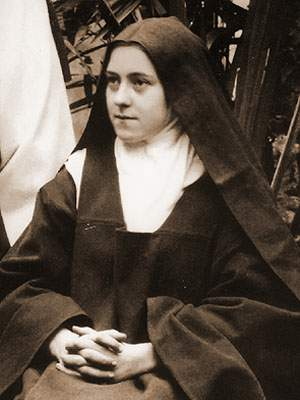
\includegraphics[scale=0.35]{theresia-2.jpg}
\end{center}
\end{floatingfigure}
Dalam autobiografinya, Theresia menyebutkan bahwa kesadaran ini mengawali kehidupannya yang baru, dimana Yesus telah menyembuhkannya dan menghilangkan sifat kepribadiannya yang buruk. Semenjak saat itu ia sadar bahwa dirinya dipenuhi oleh Roh Kudus, ia sadar bahwa ia harus mengabdikan seluruh hidupnya kepada Tuhan. Kerinduaanya untuk bersatu dengan kanak-kanak Yesus sangatlah besar dan oleh karena itulah dikemudian hari ia digelari "Santa Theresia dari Kanak-kanak Yesus". Kepada Yesus ia berjanji tidak akan pernah segan untuk melakukan apa saja yang dikehendaki Tuhan darinya. Betapa bahagia hati Theresia ketika pada umur 12 tahun ia boleh menyambut komuni untuk pertama kalinya. Dihadapan sebuah salib ia berjanji: "Yesus di kayu salib yang haus, saya akan memberikan air kepadaMu. Saya bersedia menderita sedapat mungkin agar banyak orang berdosa yang bertobat. Kerinduan Theresia yang begitu besar kepada Yesus mendesak ia untuk menjalani khusus sebagai biarawati mengikuti jejak ke 4 saudaranya yang lebih dahulu menjadi biarawati, namun ia belum bisa diterima di biara karena umurnya baru 14 tahun.

Pada umur 15 tahun saat berziarah ke Roma bersama ayahnya, Theresia dengan meminta izin khusus dari Bapa Suci agar ia diperkenankan menjadi biarawati. Permintaannya dikabulkan dan ia masuk diterima di lingkungan biara Carmelit di Lisieux Perancis.

Sembilan tahun lamanya ia hidup sebagai suster biasa, dan sebagaimana biasanya seorang suster muda, ia setiap hari melaksanakan tugas dan doa harian, harus mengatasi perasaan marah, tersinggung, iri hati, memerangi kebosanan dan berbagai ragam godaan lahir maupun batin. Untuk mencapai kesempurnaan hidup ia memilih "Jalan Sedehana" berdasarkan ajaran kitab suci yaitu hidup selaku anak kecil, penuh cinta dan iman akan kepercayaan Allah serta penyerahan diri yang total dengan penuh perasaan gembira. Demi cita-cita itu ia melakukan hal-hal kecil dan kewajiban sehari-hari di biara dengan penuh tanggung jawab karena cinta kasihnya yang besar kepada Allah Bapa di surga.

Ia sedih sekali melihat banyak orang menyakiti hati Yesus dengan berbuat dosa dan tidak mau bertobat. Untuk mempertobatkan orang-orang berdosa itu, ia mempersembahkan dirinya sebagai korban pepulih dosa-dosa. Ia rajin berdoa dan melakukan tapa bagi semua orang berdosa. Ia juga berdoa bagi para missionaris dan kemajuan kerajaan Allah di seluruh dunia.

Theresia akhirnya menderita sakit paru-paru yang sangat parah. Selama 2 tahun ia menanggung beban penderitaan itu dengan gembira. Penyakit ini kemudian merenggut nyawanya pada tanggal 30 September 1897 di biara Lisieux. Sebelum menghembuskan nafasnya ia berjanji untuk menurunkan hujan mawar ke dunia. Janji ini terpenuhi dengan banyaknya karunia Allah yang diberikan kepada semua orang yang berdoa dengan perantaranya. Theresia meninggal dalam usia yang sangat muda 24 tahun. Pada tahun 1925 ia ditetapkan sebagai "Santa" oleh Paus Pius XI (1922-1939) dan diangkat menjadi Santa pelindung negara Perancis oleh Paus Pius XII (1939-1958)

\subsubsection*{Setelah Theresia Wafat}

Setelah wafat, Theresia menjadi terkenal karena buku yang ditulisnya "Kisah Suatu Jiwa," yang diterbitkan satu tahun setelah wafatnya (di Indonesia diterjemahkan dengan judul: 'Aku Percaya akan Cinta Kasih Allah'). Theresia dikanonisasi pada tahun 1925 oleh Paus Pius X. Ia dikenal dengan sebutan Santa Theresia dari Kanak-kanak Yesus atau Santa Theresia si Bunga Kecil. St. Theresia bersama-sama dengan St. Jeanne d'Arc diberi gelar Pelindung Perancis. Selain itu St. Theresia bersama-sama dengan St. Fransiskus Xaverius diberi gelar Pelindung Misionaris.  Pada tanggal 19 Oktober 1997, Theresia juga menjadi wanita ke-3 yang diberi gelar Doktor Gereja. Kita dapat mohon bantuannya mengenai apa saja. Ia pernah berjanji  akan melimpahi kita dengan bunga-bunga mawar dari surga dan memang, sejak kematiannya banyak mukjizat yang terjadi berkat bantuan doanya. Pestanya diraya-kan setiap tanggal 1 Oktober.

\subsection*{Rahasia Theresia: Jalan Kecil, Jalan Kanak-Kanak Rohani}

\begin{floatingfigure}[l]{2.75cm}
\begin{center}
\includegraphics[scale=0.275]{theresia-3.jpg}
\end{center}
\end{floatingfigure}
Theresia seorang gadis yang sederhana dengan `jalan kecilnya' yang istimewa.  Ia menunjukkan bahwa \textbf{kekudusan dapat dicapai oleh siapa saja betapa pun rendah, hina dan biasanya orang itu}. Caranya ialah dengan melaksanakan pekerjaan-pekerjaan kecil dan tugas sehari-hari dengan penuh cinta kasih murni kepada Tuhan. Kamu pun dapat menjadi kudus dengan cara-cara sederhana seperti yang dilakukan oleh St. Theresia dengan jalan kecilnya.


\chapter[Informasi Umat]{Informasi Umat}
\section[Pengurus]{Pengurus}

\footnotesize 
\begin{center}
SUSUNAN PENGURUS LINGKUNGAN SANTA THERESIA 
\par
PERIODE TAHUN 2017 -- 2019
\end{center}
\footnotesize 
\begin{longtable}{p{0.3cm}p{3cm}p{3.5cm}p{4cm}}
\multicolumn{2}{l}{Ketua I}&Antonius Supriyana &+6285 865 355 895\\
\multicolumn{2}{l}{Ketua II}&FX. Sularto &+6281 314 190 698\\
\multicolumn{2}{l}{Sekretaris I}&M.M.S.U. Chrissumiwi &+6281 392 301 293\\
\multicolumn{2}{l}{Bendahara I}&Theresia Prima Ari Setiyani&+6285 6288 6539\\
\multicolumn{2}{l}{Bendahara II}&Agnes Sukarmi&+6281 328 795 814\\

\setcounter{nourut}{0}\\
\multicolumn{2}{l}{\textit{\textbf{Tim Kerja Liturgi}}}&&\\
&Koordinator&Yohanes Suyanto &+6285 6286 9037\\
\nexturut&Misa/Peribadatan/Doa Lingkungan &M.Th. Nanik Ismarjati&+6281 5686 1272\\
\nexturut&Koor&Maria Sode Muda&+6281 392 842 606\\
&&Valentina Isti Rudati&+6281 328 692 102\\

\setcounter{nourut}{0}\\
\multicolumn{2}{l}{\textit{\textbf{Tim Kerja Pewartaan}}}&Neo Suradi&+6281 578 115 615\\

\setcounter{nourut}{0}\\
\multicolumn{2}{l}{\textit{\textbf{Tim Kerja Kemasyarakatan}}}&&\\
&Koordinator&Cornelius Triyono &+6281 578 179 267\\
\nexturut&Tabungan Cinta Kasih (TCK)&Kristina Tri Tutwuri &+6281 2275 2803\\
\nexturut&Prolenan&Roselina Zeli Puspitasari &\\
\nexturut&Pangruktilaya&M. Th. Nanik Ismarjati&+6281 5686 1272\\
&&C. Prihatiningtyas&+6287 838 4523\\
\nexturut&PSE&Yohanes Sudarmadi&+6281 328 450 101\\
\nexturut&Majalah Paroki/Lingkungan&OMK Lingkungan&\\

\setcounter{nourut}{0}\\
\multicolumn{2}{l}{\textit{\textbf{Bidang Paguyuban}}}&&\\
&Koordinator&Aloysius Heru Pratomo&+6281 328 259 725\\
\nexturut&Pag. Ibu-ibu Lingkungan&Anastasia Sri Supriyati&+62 813 2845 0101\\
\nexturut&Pag. OMK Lingkungan&Maria Regina Tri Marieska&+62 813 9205 4103\\
\nexturut&Pendamping OMK Lingk.&Andreas Keso Muda&+6281 328 692 102\\

\setcounter{nourut}{0}\\
\multicolumn{2}{l}{\textit{\textbf{Bidang Rumah Tangga}}}&&\\
&Koordinator&Yohanes Djoko Marsito&+62 858 2013 3321\\
\nexturut&Paramenta&Yohanes Suyanto&+6285 6286 9037\\
\nexturut&Tata Bunga&C. Prihatiningtyas S.&+6287 838 452 319\\
&&M.M.S.U.Chrissumiwi&+6281 392 301 293\\


\setcounter{nourut}{0}\\
\multicolumn{2}{l}{\textit{\textbf{Litbang dan Data umat}}}&&\\
&&Andreas Keso Muda&\\
&&Yohanes Suyanto&\\
\end{longtable}

\section{Data Umat}

DATA KELUARGA UMAT LINGKUNGAN SANTO PETRUS
\setcounter{nourut}{0}

\begin{longtable}{|p{1cm}|p{3cm}|>{\raggedright}p{3.5cm}|p{2.1cm}|C{0.5cm}|C{0.5cm}|C{0.5cm}|}
\hline
\centering No &
\centering Nama \par Kepala Keluarga &
\centering Alamat &
\centering Telepon &
\multicolumn{3}{m{1.5cm}|}{\centering Anggota\par
Keluarga}\\[-0.75em] \cline{5-7}
 &
 &
 &
 &
\centering L&
\centering P &
Jml \\
\hline
\endhead
\hline
\endfoot

\centering\nexturut&Aloysius Lamakey&Pugeran - Gg. Nilam No. 6&81328034283&1&2&3\\\hline
\centering\nexturut&Anggara Pramudita, Domitianus&Jl. Utama Pugeran&8175468228&1&2&3\\\hline
\centering\nexturut&Ariwibowo Sudaryanto, Fransiskus Xaverius&Pugeran - Jl. Utama&85867335678&1&1&2\\\hline
\centering\nexturut&Baharudin, Thomas&Pugeran - RT.21 RW. 64 Gg. Bimo&81392842606&1&2&3\\\hline
\centering\nexturut&Dalyono, Valentinus&Sombomerten 06, RW 21&81932601029&2&2&4\\\hline
\centering\nexturut&Djarot Sadharto Widiatmoko, Michael Robertus&Jl. Lele I/7 Pugeran, Maguwoharjo, Depok, Sleman, Yogyakarta&6287751024663&3&1&4\\\hline
\centering\nexturut&Djoko Marsito, Yohanes&Pugeran, Maguwoharjo&85820133321&1&2&3\\\hline
\centering\nexturut&Gelungminangkoro Widyanurcahyo, Dominikus&Jl Utama 110 Pugeran Maguwoharjo&81328624116&1&2&3\\\hline
\centering\nexturut&Heru Pratomo, Aloysius&Sombomerten RT06/RW21 Maguwoharjo, Depok, Sleman&6281328259725&1&0&1\\\hline
\centering\nexturut&Keso Muda, Andreas&Pugeran - RT 02 RW 64 Gg. Bima No 27&81328692102&1&3&4\\\hline
\centering\nexturut&Krisni Prihartati, Cornelia&Pugeran - Jl. Utama&0274-4333615; 08574335162&0&2&2\\\hline
\centering\nexturut&Mardi Susanti, Agustina&Pugeran - RT.07 RW.65 Jl. Puger V No 2&8164229555&0&1&1\\\hline
\centering\nexturut&Nanik Ismarjati, Maria Theresia&Sombomerten - RT.06 RW. 21 Gg. Sadewo 185 &81568612272&0&1&1\\\hline
\centering\nexturut&Niha Lamakey, Yakobus&Pugeran - Gg. Nilam No. 6&0274 7839098&2&1&3\\\hline
\centering\nexturut&Sandi Ignatius&Pugeran - RT.02 RW.64 &85292171946&1&2&3\\\hline
\centering\nexturut&Saptanto Sarwo Basuki, Yohanes&Jl. Puger Utama, Gg Perkutut No. 8 B, Pugeran, Maguwoharjo, Depok, Sleman&6281373249666&3&2&5\\\hline
\centering\nexturut&Setyawan Putra, Thomas&Pugeran, Jl. Jupiter I No.9, Maguwoharjo&82138125680&3&2&5\\\hline
\centering\nexturut&Sudarmadi, Yohanes&Pugeran, Jl. Pugeran Utama No. 66, Maguwoharjo&0274 4333545&1&1&2\\\hline
\centering\nexturut&Sujarwanto, Agustinus&Pugeran- RT.09 RW.065 Jl. Pugeran Utama&8157955674&2&1&3\\\hline
\centering\nexturut&Sularto, Fransiscus Xaverius&Pugeran - RT.04 RW. 09 Jl. Lele I No 4&81314190698&1&1&2\\\hline
\centering\nexturut&Sunaryo Prononagoro Kra, Yohanes Pemandi&Pugeran- RT 17 RW. 65 Jl. Perkutut&0274 7400625&1&3&4\\\hline
\centering\nexturut&Supriadi, Cornelius&Pugeran, Jl. Perkutut Komp. Batan&0274 7497125&2&2&4\\\hline
\centering\nexturut&Suprihatin, Kristina&Pugeran - RT.10 RW 64 Jl. Merpati No 1&81568052255&0&2&2\\\hline
\centering\nexturut&Supriyana, Antonius&Jl. Utama Pugeran&85865355895&2&2&4\\\hline
\centering\nexturut&Suradi, Neo&Pugeran - RT.10 RW.64, Maguwoharjo&0274 556180&1&2&3\\\hline
\centering\nexturut&Suripto, Yohanes&Pugeran Gg. Nilam No. 4&817889303&2&1&3\\\hline
\centering\nexturut&Suroyo, Paulus&Pugeran - RT.03 RW.09 Gg. Bawal&8122752803&2&2&4\\\hline
\centering\nexturut&Suyanto, Yohanes&Sombomerten - RT.06 RW.21&0274-4333886&4&2&6\\\hline
\centering\nexturut&Temon Siswo Utomo, Margaretha&Pugeran - RT.09 RW.65&&0&1&1\\\hline
\centering\nexturut&Triyono, Cornelius&Pugeran - RT 003 RW 009 - Jl. Utama, Gg. Bawal, Maguwoharjo&81578179267&2&2&4\\\hline

\hline
\multicolumn{4}{|m{9.796cm}|}{\centering Jumlah Umat} & 
\centering \jumlahL &
\centering \jumlahP &
\centering\arraybslash \jumlahLP\\ \hline
\end{longtable}

\section[Remaja dan Mudika]{Daftar Remaja dan Orang Muda Katolik (OMK) Lingkungan St. Theresia}
\begin{flushleft}
\setcounter{nourut}{0}

\begin{longtable}{|m{0.5cm}|m{3cm}|m{1.1cm}|>{\raggedright}m{3.9cm}|m{2.5cm}|}
\hline
\multirow{2}{0.5cm}{\centering No} &
\multirow{2}{3.5cm}{\centering Nama} &
\multirow{2}{1.1cm}{\centering Tahun Lahir} &
\multicolumn{2}{m{5.5cm}|}{\centering Orangtua}\\ \cline{4-5}
 & & &
\centering Nama \& Alamat &
\centering\arraybslash Telpon\\ \hline
\endhead

\centering \nexturut &	Fabiano Agiano, Cornellius	&	2006	&	Sujarwanto, Agustinus	Kusdayarti, Anastasia	-	Pugeran- Rt.09 Rw.065 Jl. Pugeran Utama	&	8157955674\\ \hline
\centering \nexturut &	Aditya Riani Widwianingrum, Stephanie	&	2006	&	Suroyo, Paulus	Tri Tutwuri, Kristina	-	Pugeran - Rt.03 Rw.09 Gg. Bawal	&	8122752803\\
\hline
\centering \nexturut &	Hargyan Revano, Petrus Krisologus	&	2004	&	Saptanto Sarwo Basuki, Yohanes	Isti Rudati, Valentina	-	Jl. Puger Utama, Gg Perkutut No. 88, Pugeran, Magu...	&	6281373249666\\
\hline
\centering \nexturut &	Rosa Firanti, Maria	&	2004	&	Suyanto, Yohanes	Prima Ari Setiyani, Theresia	-	Sombomerten - Rt.06 Rw.21	&	0274-4333886\\
\hline
\centering \nexturut &	Apriliana Wulandari, Herminigilda & 2002 & Sunaryo Prononagoro Kra, Yohanes Pemandi \par  Pugeran- RT 17 RW. 65 Jl. Perkutut & 0274 7400625 \\ \hline 
\centering \nexturut &	Aurel Dwi Irawan Putra, Fabianus & 2001 & Setyawan Putra, Thomas \par  Pugeran, Jl. Jupiter I No.9, Maguwoharjo & 082138125680 \\ \hline 
\centering \nexturut &	Desicea Calista, Redempta & 1999 & Saptanto Sarwo Basuki, Yohanes \par  Jl. Puger Utama, Gg Perkutut No. 88, Pugeran, Maguwoharjo, Depok, Sleman & +6281373249666 \\ \hline 
\centering \nexturut &	Widiastuti, Sisilia & 1999 & Suprihatin, Kristina \par  Pugeran - RT.10 RW 64 Jl. Merpati No 1 & 081568052255 \\ \hline 
\centering \nexturut &	Krissanti Dewi Danudibroto, Emerentiana & 1998 & Krisni Prihartati, Cornelia \par  Pugeran - Jl. Utama & 0274-4333615; 08574335162 \\ \hline 
\centering \nexturut &	Oldi Kristianto, Eduardus & 1998 & Suyanto, Yohanes \par  Sombomerten - RT.06 RW.21 & 0274-4333886 \\ \hline 
\centering \nexturut &	Sinar Mas Putra Pratama, Damasus & 1998 & Triyono, Cornelius \par  Pugeran - RT 003 RW 009 - Jl. Utama, Gg. Bawal, Maguwoharjo & 081578179267 \\ \hline 
\centering \nexturut &	Pratama Krisna Bayu Aji, Stefanus & 1997 & Suroyo, Paulus \par  Pugeran - RT.03 RW.09 Gg. Bawal & 08122752803 \\ \hline 
\centering \nexturut &	Titisari, Lusia & 1997 & Banarudin, Thomas \par  Pugeran - RT.21 RW. 64 Gg. Bimo & 085868421306 \\ \hline 
\centering \nexturut &	Delphito Nugroho, Bartolomeus & 1997 & Suyanto, Yohanes \par  Sombomerten - RT.06 RW.21 & 0274-4333886 \\ \hline 
\centering \nexturut &	Sode Muda Valentia, Eleonora & 1996 & Keso Muda, Andreas \par  Pugeran - RT 02 RW 64 Gg. Bima No 27 & 081328692102 \\ \hline 
\centering \nexturut &	Irawan Putramas, Tera & 1995 & Setyawan Putra, Thomas \par  Pugeran, Jl. Jupiter I No.9, Maguwoharjo & 082138125680 \\ \hline 
\centering \nexturut &	Iglia Lucya, Paulina & 1995 & Sandi Ignatius \par  Pugeran - RT.02 RW.64  & 085292171946 \\ \hline 
\centering \nexturut &	Stanley Andi Pradana, Ignatius & 1994 & Saptanto Sarwo Basuki, Yohanes \par  Jl. Puger Utama, Gg Perkutut No. 88, Pugeran, Maguwoharjo, Depok, Sleman & +6281373249666 \\ \hline 
\centering \nexturut &	Melati, Rosevita & 1994 & Suradi, Neo \par  Pugeran - RT.10 RW.64, Maguwoharjo & 0274 556180 \\ \hline 
\centering \nexturut &	Sadewa Setyanta, Pascalis & 1993 & Suyanto, Yohanes \par  Sombomerten - RT.06 RW.21 & 0274-4333886 \\ \hline 
\centering \nexturut &	Aditya Bimantara, Andreas & 1993 & Supriadi, Cornelius \par  Pugeran, Jl. Perkutut Komp. Batan & 0274 7497125 \\ \hline 
\centering \nexturut &	Emerita Davita, Rosalinda & 1991 & Supriyana, Antonius \par  Pugeran & 085865355895 \\ \hline 
\centering \nexturut &	Edlina Adiaty, Clara & 1991 & Supriadi, Cornelius \par  Pugeran, Jl. Perkutut Komp. Batan & 0274 7497125 \\ \hline 
\centering \nexturut &	Regina Tri Marieska, Maria & 1989 & Djoko Marsito, Yohanes \par  Pugeran, Maguwoharjo & 085820133321 \\ \hline 
\centering \nexturut &	Febrianto, Dominik & 1987 & Suripto, Yohanes \par  Pugeran Gg. Nilam No. 4 & 0817889303 \\ \hline 
\centering \nexturut &	Amarylis Illona Muda, Maria & 1987 & Keso Muda, Andreas \par  Pugeran - RT 02 RW 64 Gg. Bima No 27 & 081328692102 \\ \hline 
\centering \nexturut &	Lamakey Maria Anastasia Bare & 1985 & Aloysius Lamakey \par  Pugeran - Gg. Nilam No. 6 & 081328034283 \\ \hline 

\end{longtable}
\end{flushleft}

\section[Jadwal Kegiatan]{Jadwal Kegiatan}
JADWAL KEGIATAN DOA LINGKUNGAN ST. THERESIA 2015


\begin{flushleft}
\scriptsize
\begin{longtable}{|m{1.2cm}|m{0.4cm}|m{0.9cm}|m{2.6cm}|m{2.1cm}|m{1.5cm}|m{3.1cm}|}
\hline
\centering \textbf{Bulan} &
\centering \textbf{Tgl} &
\centering \textbf{Hari} &
\centering \textbf{Bacaan} &
\centering \textbf{Acara} &
\centering \textbf{Tempat} &
\centering\arraybslash \textbf{Petugas}\\ \hline
\endhead
\hline
\endfoot
Januari& 6& Rabu& 1Yoh. 4:11-18,Mzm. 72:1-2,10-11,12-13,Mrk. 6:45-52& Natalan Lingkungan& Joglo Lawas& Prodiakon\par Anton Supriyana\\ 	\cline{2-7}
& 28& Kamis& 2Sam. 11:1-4a,5-10a,13-17,Mzm. 51:3-4,5-6a,6bc-7,10-11,Mrk. 4:26-34& Doa Lingkungan& C. Triyono& Suyanto, Yohanes\par Titisari, Lusia\\ 	\hline
Februari& 11& Kamis& Yl. 2:12-18,Mzm. 51:3-4,5-6a,12-13,14,17,2Kor. 5:20-6:2,Mat. 6:1-6,16-18& Doa Lingkungan& Y. Suripto& Anton Supriyana\par C. Triyono\\ 	\cline{2-7}
& 18& Kamis& Yun. 3:1-10,Mzm. 51:3-4,12-13,18-19,Luk. 11:29-32& Prapaskah I& P. Suroyo& Tim\par \\ 	\cline{2-7}
& 25& Kamis& Yer. 18:18-20,Mzm. 31:5-6,14,15-16,Mat. 20:17-28& Prapaskah II& P. Suroyo& Tim\par \\ 	\hline
Maret& 3& Kamis& Yer. 7:23-28,Mzm. 95:1-2,6-7,8-9,Luk. 11:14-23& Prapaskah III& P. Suroyo& Tim\par \\ 	\cline{2-7}
& 10& Kamis& Kel. 32:7-14,Mzm. 106:19-20,21-22,23,Yoh. 5:31-47& Prapaskah IV& P. Suroyo& Tim\par \\ 	\cline{2-7}
& 17& Kamis& Dan. 3:14-20,24-25,28,Dan. 3:52,53,54,55,56,Yoh. 8:31-42& Prapaskah V& P. Suroyo& Tim\par \\ 	\hline
April& 7& Kamis& Kis. 5:17-26,Mzm. 34:2-3,4-5,6-7,8-9,Yoh. 3:16-21& Paskahan Lingkungan& Joglo Lawas& Prodiakon\par Sode Muda, Maria\\ 	\cline{2-7}
& 21& Kamis& Kis. 13:13-25,Mzm. 89:2-3,21-22,25,27,Yoh. 13:16-20& Doa Lingkungan& Aloysius Lamakey& Nanik Ismarjati, Maria Theresia\par Sri Utami Chrisssumiwi, Margareta Maria\\ 	\hline
Mei& 1& Minggu& Kis. 15:1-2,22-29,Mzm. 67:2-3,5,6,8,Why. 21:10-14.22-23,Yoh. 14:23-29,Kis. 20:17-38,& Rosario& Joglo Lawas& Aloysius Lamakey\par Sode Muda, Maria\\ 	\cline{2-7}
& 2& Senin& Kis. 16:11-15,Mzm. 149:1-2,3-4,5-6a,9b,Yoh. 15:26-16:4a,Kis. 21:1-26,& Rosario& Joglo Lawas& C. Triyono\par Aloysius Lamakey\\ 	\cline{2-7}
& 3& Selasa& 1Kor. 15:1-8,Mzm. 19:2-3,4-5,Yoh. 14:6-14,Why. 18:21,19:10,& Rosario& Joglo Lawas& Sode Muda, Maria\par Tri Tutwuri, Kristina\\ 	\cline{2-7}
& 4& Rabu& Kis. 17:15,22-18:1,Mzm. 148:1-2,11-12ab,12c-14a,14bcd,Yoh. 16:12-15,Kis. 21:40-22:21,& Rosario& Joglo Lawas& Sri Supriyati, Anastasia\par Lamakey Maria Antonia Tona\\ 	\cline{2-7}
& 5& Kamis& Kis. 1:1-11,Mzm. 47:2-3,6-7,8-9,Ef. 1:17-23,Ibr. 9:24-28; 10:19-23,Luk. 24:46-53,Ef 4:1-24,& Rosario& Joglo Lawas& Pratama Krisna Bayu Aji, Stefanus\par Suyanto, Yohanes\\ 	\cline{2-7}
& 6& Jumat& Kis. 18:9-18,Mzm. 47:2-3,4-5,6-7,Yoh. 16:20-23a,Kis. 22:22-23:11,& Rosario& Joglo Lawas& Sularto, Fransiscus Xaverius\par Nanik Ismarjati, Maria Theresia\\ 	\cline{2-7}
& 7& Sabtu& Kis. 18:23-28,Mzm. 47:2-3,8-9,10,Yoh. 16:23b-28,Kis. 23:12-35,& Rosario& Joglo Lawas& Budi Hartuti, Maria Goreti\par Agnes Sukarmi\\ 	\cline{2-7}
& 8& Minggu& Kis. 7:55-60,Mzm. 97:1,2b,6,7c,9,Why. 22:12-14,16-17,20,Yoh. 17:20-26,Kis. 24:1-6,8b-27,& Rosario& Joglo Lawas& Lamakey Maria Antonia Tona\par Zeli Puspitasari, R\\ 	\cline{2-7}
& 9& Senin& Kis. 19:1-8,Mzm. 68:2-3,4-5ac,6-7ab,Yoh. 16:29-33,Kis. 25:1-27,& Rosario& Joglo Lawas& Arie Wibowo S, FX\par Sudarmadi, Yohanes\\ 	\cline{2-7}
& 10& Selasa& Kis. 20:17-27,Mzm. 68:10-11,20-21,Yoh. 17:1-11a,Kis. 26:1-32,& Rosario& Joglo Lawas& Apriliana Wulandari, Herminigilda\par Sandi Ignatius\\ 	\cline{2-7}
& 11& Rabu& Kis. 20:28-38,Mzm. 68:29-30,33-35a,35b-36c,Yoh. 17:11b-19,Kis. 27:1-20,& Rosario& Joglo Lawas& Jatiningsih, Yulia\par Budi Hartuti, Maria Goreti\\ 	\cline{2-7}
& 12& Kamis& Kis. 22:30; 23:6-11,Mzm. 16:1-2a,5,7-8,9-10,11,Yoh. 17:20-26,Kis. 27:21-44,& Rosario& Joglo Lawas& Prima Ari Setiyani, Theresia\par Titisari, Lusia\\ 	\cline{2-7}
& 13& Jumat& Kis. 25:13b-21,Mzm. 103:1-2,11-12,19-20ab,Yoh. 21:15-19,Kis. 28:1-14,& Rosario& Joglo Lawas& Sudarmadi, Yohanes\par Apriliana Wulandari, Herminigilda\\ 	\cline{2-7}
& 14& Sabtu& Kis. 1:15-17,20-26,Mzm. 113:1-2,3-4,5-6,7-8,Yoh. 15:9-17,Kis. 5:12-32,1Kor. 1:17-2:5,1Kor. 4:1-16,& Rosario& Joglo Lawas& Djuwarni Anastasia Hedwig\par Anton Supriyana\\ 	\cline{2-7}
& 15& Minggu& Kis. 2:1-11,Mzm. 104:1ab,24ac,29bc-30,31,34,1Kor. 12:3b-7,12-13,Rm. 8:8-17,Yoh. 14:15-16,23b-26,Rm. 8:5-27,& Rosario& Joglo Lawas& Lamakey Maria Anastasia Bare\par Lamakey Maria Anastasia Bare\\ 	\cline{2-7}
& 16& Senin& Yak. 3:13-18,Mzm. 19:8,9,10,15,Mrk. 9:14-29,2Kor. 1:15-2:11,& Rosario& Joglo Lawas& Sri Utami Chrisssumiwi, Margareta Maria\par Arie Wibowo S, FX\\ 	\cline{2-7}
& 17& Selasa& Yak. 4:1-10,Mzm. 55:7-8,9-10a,10b-11a,10b-11a,23,Mrk. 9:30-37,2Kor. 2:12-3:6,& Rosario& Joglo Lawas& Djoko Marsito, Yohanes\par Melati, Rosevita\\ 	\cline{2-7}
& 18& Rabu& Yak. 4:13-17,Mzm. 49:2-3,6-7,8-10,11,Mrk. 9:38-40,2Kor. 3:7-4:4,& Rosario& Joglo Lawas& Sandi Ignatius\par Pratama Krisna Bayu Aji, Stefanus\\ 	\cline{2-7}
& 19& Kamis& Yak. 5:1-6,Mzm. 49:14-15ab,15cd-16,17-18,19-20,Mrk. 9:41-50,2Kor. 4:5-18,& Rosario& Joglo Lawas& Nanik Ismarjati, Maria Theresia\par Djoko Marsito, Yohanes\\ 	\cline{2-7}
& 20& Jumat& Yak. 5:9-12,Mzm. 103:1-2,3-4,8-9,11-12,Mrk. 10:1-12,2Kor. 5:1-21,& Rosario& Joglo Lawas& Tri Tutwuri, Kristina\par Sri Utami Chrisssumiwi, Margareta Maria\\ 	\cline{2-7}
& 21& Sabtu& Yak. 5:13-20,Mzm. 141:1-2,3,8,Mrk. 10:13-16,2Kor. 6:1-7:1,& Rosario& Joglo Lawas& Chatarina Sukarmi\par Prima Ari Setiyani, Theresia\\ 	\cline{2-7}
& 22& Minggu& Ams. 8:22-31,Mzm. 8:4-5,6-7,8-9,Rm. 5:1-5,Yoh. 16:12-15,Ef 1:1-14,1Kor 2:1-16,& Rosario& Joglo Lawas& Tri Susilowati, Caecilia\par Djuwarni Anastasia Hedwig\\ 	\cline{2-7}
& 23& Senin& 1Ptr. 1:3-9,Mzm. 111:1-2,5-6,9,10c,Mrk. 10:17-27,2Kor. 8:1-24,& Rosario& Joglo Lawas& Setya Prihatiningtyas, Chatarina\par Tri Susilowati, Caecilia\\ 	\cline{2-7}
& 24& Selasa& 1Ptr. 1:10-16,Mzm. 98:1,2-3ab,3c-4,Mrk. 10:28-31,2Kor. 9:1-15,& Rosario& Joglo Lawas& Titisari, Lusia\par Setya Prihatiningtyas, Chatarina\\ 	\cline{2-7}
& 25& Rabu& 1Ptr. 1:18-25,Mzm. 147:12-13,14-15,19-20,Mrk. 10:32-45,2Kor. 10:1-11:6,& Rosario& Joglo Lawas& Zeli Puspitasari, R\par Sularto, Fransiscus Xaverius\\ 	\cline{2-7}
& 26& Kamis& 1Ptr. 2:2-5,9-12,Mzm. 100:2,3,4,5,Mrk. 10:46-52,2Kor. 11:7-29,& Rosario& Joglo Lawas& Supriadi, Cornelius\par Sode Muda Valentia, Elenora\\ 	\cline{2-7}
& 27& Jumat& 1Ptr. 4:7-13,Mzm. 96:10,11-12,13,Mrk. 11:11-26,2Kor. 11:30,12:13,& Rosario& Joglo Lawas& Sukarmi, Agnes\par Suradi, Neo\\ 	\cline{2-7}
& 28& Sabtu& Yud. 17:20b-25,Mzm. 63:2,3-4,5-6,Mrk. 11:27-33,2Kor. 12:14-13:14,& Rosario& Joglo Lawas& Sode Muda Valentia, Elenora\par Keso Muda, Andreas\\ 	\cline{2-7}
& 29& Minggu& Kej. 14:18-20,Mzm. 110:1,2,3,4,1Kor. 11:23-26,Luk. 9:11b-17,Rm. 5:1-21,Kel. 24:1-11,& Rosario& Joglo Lawas& Melati, Rosevita\par Sri Supriyati, Anastasia\\ 	\cline{2-7}
& 30& Senin& 2Ptr. 1:1-7,Mzm. 91:1-2,14-15ab,15c-16,Mrk. 12:1-12,Gal. 1:13-2:10,& Rosario& Joglo Lawas& Suradi, Neo\par Jatiningsih, Yulia\\ 	\cline{2-7}
& 31& Selasa& Zef. 3:14-18a,Rm. 12:9-16b,Yes. 12:2-3,4,Luk. 1:39-56,Kid. 2:8-14; 8:6-7,& Rosario& Joglo Lawas& Suyanto, Yohanes\par Supriadi, Cornelius\\ 	\hline
Juni& 9& Kamis& 1Raj. 18:41-46,Mzm. 65:10abcd,10e-11,12-13,Mat. 5:20-26& Doa Lingkungan& Y. Djoko Marsito& Neo Suradi\par Nanik Ismarjati, Maria Theresia\\ 	\cline{2-7}
& 23& Kamis& 2Raj. 24:8-17,Mzm. 79:1-2,3-5,8,9,Mat. 7:21-29& Doa Lingkungan& Y. Sudarmadi& Heru Pratomo, Aloysius\par Prima Ari Setiyani, Theresia\\ 	\hline
Juli& 14& Kamis& Yes. 26:7-9,12,16-19,Mzm. 102:13-14ab,15,16-18,19-21,Mat. 11:28-30& Doa Lingkungan& FX Arie WS& Djoko Marsito, Yohanes\par Sode Muda Valentia, Elenora\\ 	\cline{2-7}
& 28& Kamis& Yer. 18:1-6,Mzm. 146:2abc,2d-4,5-6,Mat. 13:47-53& Doa Lingkungan& Andre Keso Muda& Aloysius Lamakey\par Sode Muda, Maria\\ 	\hline
Agustus& 11& Kamis& Yeh. 12:1-12,Mzm. 78:56-57,58-59,61-62,Mat. 18:21,19:1& Doa Lingkungan& Th. Banar& Anton Supriyana\par C. Triyono\\ 	\cline{2-7}
& 25& Kamis& Why. 21:9b-14,Mzm. 145:10-11,12-13ab,17-18,Yoh. 1:45-51& Doa Lingkungan& Ig. Sandy& Suyanto, Yohanes\par Tri Tutwuri, Kristina\\ 	\hline
September& 1& Kamis& 1Kor. 3:18-23,Mzm. 24:1-2,3-4ab,5-6,Luk. 5:1-11& BKSN I& Y. Suyanto& Tim\par \\ 	\cline{2-7}
& 8& Kamis& Mi. 5:1-4a,Rm. 8:28-30,Mzm. 13:6ab,6cd,Mat. 1:1-16& BKSN II& Y. Suyanto& Tim\par \\ 	\cline{2-7}
& 15& Kamis& Bil. 21:4-9,Mzm. 78:1-2,34-35,36-37,38,Flp. 2:6-11,Yoh. 3:13-17& BKSN III& Y. Suyanto& Tim\par \\ 	\cline{2-7}
& 22& Kamis& Pkh. 1:2-11,Mzm. 90:3-4,5-6,12-13,14,17,Luk. 9:7-9& BKSN IV& Y. Suyanto& Tim\par \\ 	\hline
Oktober& 1& Sabtu& Ayb. 42:1-3,5-6,12-17,Mzm. 119:66,71,75,91,125,130,Luk. 10:17-24,. atau:,Yes. 66:10-14b,1Kor. 12:31,13:13;,Mat. 18:1-4,2Taw. 29:1-2; 30:1-16a,& Rosario& Joglo Lawas& Nanik Ismarjati, Maria Theresia\par Melati, Rosevita\\ 	\cline{2-7}
& 2& Minggu& Hab. 1:2-3; 2:2-4,Mzm. 95:1-2,6-7,8-9,2Tim. 1:6-8,13-14,Luk. 17:5-10,Sir. 1:1-20,& Rosario& Joglo Lawas& Sularto, Fransiscus Xaverius\par Tri Tutwuri, Kristina\\ 	\cline{2-7}
& 3& Senin& Gal. 1:6-12,Mzm. 111:1-2,7-8,9,10c,Luk. 10:25-37,Sir. 2:1-18,& Rosario& Joglo Lawas& Tri Susilowati, Caecilia\par Keso Muda, Andreas\\ 	\cline{2-7}
& 4& Selasa& Gal. 1:13-24,Mzm. 139:1-3,13-14ab,14c-15,Luk. 10:38-42,Sir. 3:1-16,& Rosario& Joglo Lawas& Suradi, Neo\par Agnes Sukarmi\\ 	\cline{2-7}
& 5& Rabu& Gal. 2:1-2,7-14,Mzm. 117:1,2,Luk. 11:1-4,Sir. 3:17-4:10,& Rosario& Joglo Lawas& Sudarmadi, Yohanes\par Apriliana Wulandari, Herminigilda\\ 	\cline{2-7}
& 6& Kamis& Gal. 3:1-5,Luk. 1:69-70,71-72,73-75,Luk. 11:5-13,Sir. 5:1-6:4,& Rosario& Joglo Lawas& Melati, Rosevita\par Suradi, Neo\\ 	\cline{2-7}
& 7& Jumat& Gal. 3:7-14,Mzm. 111:1-2,3-4,5-6,Luk. 11:15-26,Sir. 6:5-37,& Rosario& Joglo Lawas& Arie Wibowo S, FX\par Sri Supriyati, Anastasia\\ 	\cline{2-7}
& 8& Sabtu& Gal. 3:22-29,Mzm. 105:2-3,4-5,6-7,Luk. 11:27-28,Sir. 7:22-36,& Rosario& Joglo Lawas& Lamakey Maria Anastasia Bare\par Titisari, Lusia\\ 	\cline{2-7}
& 9& Minggu& 2Raj. 5:14-17,Mzm. 98:1,2-3ab,3cd-4,2Tim. 2:8-13,Luk. 17:11-19,Sir. 10:6-18,& Rosario& Joglo Lawas& Apriliana Wulandari, Herminigilda\par Setya Prihatiningtyas, Chatarina\\ 	\cline{2-7}
& 10& Senin& Gal. 4:22-24,26-27,31-5:1,Mzm. 113:1-2,3-4,5a,6-7,Luk. 11:29-32,Sir. 11:11-28,& Rosario& Joglo Lawas& Suyanto, Yohanes\par Sode Muda Valentia, Elenora\\ 	\cline{2-7}
& 11& Selasa& Gal. 4:31b,5:6;,Mzm. 119:41,43,44,45,47,48,Luk. 11:37-41,Sir. 14:20-15:10,& Rosario& Joglo Lawas& Aloysius Lamakey\par Suyanto, Yohanes\\ 	\cline{2-7}
& 12& Rabu& Gal. 5:18-25,Mzm. 1:1-2,3,4,6,Luk. 11:42-46,Sir. 15:11-20,& Rosario& Joglo Lawas& Prima Ari Setiyani, Theresia\par Budi Hartuti, Maria Goreti\\ 	\cline{2-7}
& 13& Kamis& Ef. 1:1-10,Mzm. 98:1,2-3ab,3cd-4,5-6,Luk. 11:47-54,Sir. 16:24-17:14,& Rosario& Joglo Lawas& Sri Utami Chrisssumiwi, Margareta Maria\par Sularto, Fransiscus Xaverius\\ 	\cline{2-7}
& 14& Jumat& Ef. 1:11-14,Mzm. 33:1-2,4-5,12-13,Luk. 12:1-7,Sir. 17:15-32,& Rosario& Joglo Lawas& Titisari, Lusia\par Zeli Puspitasari, R\\ 	\cline{2-7}
& 15& Sabtu& Ef. 1:15-23,Mzm. 8:2-3a,4-5,6-7,Luk. 12:8-12,Sir. 24:1-22,& Rosario& Joglo Lawas& Supriadi, Cornelius\par Tri Susilowati, Caecilia\\ 	\cline{2-7}
& 16& Minggu& Kel. 17:8-13,Mzm. 121:1-2,3-4,5-6,7-8,2Tim. 3:14-4:2,Luk. 18:1-8,Sir. 26:1-4,9-18,& Rosario& Joglo Lawas& Jatiningsih, Yulia\par Nanik Ismarjati, Maria Theresia\\ 	\cline{2-7}
& 17& Senin& Ef. 2:1-10,Mzm. 100:2,3,4,5,Luk. 12: 13-21,Sir. 27:22-28:7,& Rosario& Joglo Lawas& Sode Muda, Maria\par Sri Utami Chrisssumiwi, Margareta Maria\\ 	\cline{2-7}
& 18& Selasa& 2Tim. 4:10-17b,Mzm. 145:10-11,12-13ab,17-18,Luk. 10:1-9,Kis. 9:27-31; 11:19-26,& Rosario& Joglo Lawas& Setya Prihatiningtyas, Chatarina\par Sandi Ignatius\\ 	\cline{2-7}
& 19& Rabu& Ef. 3:2-12,Yes. 12:2-3,4bcd,5-6,Luk. 12:39-48,Sir. 35:1-17,& Rosario& Joglo Lawas& Zeli Puspitasari, R\par Aloysius Lamakey\\ 	\cline{2-7}
& 20& Kamis& Ef. 3:14-21,Mzm. 33:1-2,4-5,11-12,18-19,Luk. 12:49-53,Sir. 38:24-39:11,& Rosario& Joglo Lawas& C. Triyono\par Sode Muda, Maria\\ 	\cline{2-7}
& 21& Jumat& Ef. 4:1-6,Mzm. 24:1-2,3-4ab,5-6,Luk. 12:54-59,Sir. 42:15-25; 43:27-33,& Rosario& Joglo Lawas& Sri Supriyati, Anastasia\par Jatiningsih, Yulia\\ 	\cline{2-7}
& 22& Sabtu& Ef. 4:7-16,Mzm. 122:1-2,3-4a,4b-5,Luk. 13:1-9,Hab. 2:5-20,& Rosario& Joglo Lawas& Budi Hartuti, Maria Goreti\par Prima Ari Setiyani, Theresia\\ 	\cline{2-7}
& 23& Minggu& Sir. 35:12-14,16-18,Mzm. 34:2-3,17-18,19,23,2Tim. 4:6-8,16-18,Luk. 18:9-14,Keb. 1:1-15,& Rosario& Joglo Lawas& Sukarmi, Agnes\par Lamakey Maria Anastasia Bare\\ 	\cline{2-7}
& 24& Senin& Ef. 4:32-5:8,Mzm. 1:1-2,3,4,6,Luk. 13:10-17,Keb. 1:16-2:24,& Rosario& Joglo Lawas& Tri Tutwuri, Kristina\par Djoko Marsito, Yohanes\\ 	\cline{2-7}
& 25& Selasa& Ef. 5:21-33,Mzm. 128:1-2,3,4-5,Luk. 13:18-21,Keb. 3:1-19,& Rosario& Joglo Lawas& Sandi Ignatius\par Pratama Krisna Bayu Aji, Stefanus\\ 	\cline{2-7}
& 26& Rabu& Ef. 6:1-9,Mzm. 145:10-11,12-13ab,13cd-14,Luk. 13:22-30,Keb. 4:1-20,& Rosario& Joglo Lawas& Lamakey Maria Antonia Tona\par Lamakey Maria Antonia Tona\\ 	\cline{2-7}
& 27& Kamis& Ef. 6:10-20,Mzm. 144:1,2,9-10,Luk. 13:31-35,Keb. 5:1-23,& Rosario& Joglo Lawas& Pratama Krisna Bayu Aji, Stefanus\par Sudarmadi, Yohanes\\ 	\cline{2-7}
& 28& Jumat& Ef. 2:19-22,Mzm. 19:2-3,4-5,Luk. 6:12-19,Kis. 5:12-32,1Kor. 1:17-2:5,1Kor. 4:1-16,& Rosario& Joglo Lawas& Chatarina Sukarmi\par Djuwarni Anastasia Hedwig\\ 	\cline{2-7}
& 29& Sabtu& Flp. 1:18b-26,Mzm. 42:2,3,5bcd,Luk. 14:1,7-11,Keb. 7:15-30,& Rosario& Joglo Lawas& Sode Muda Valentia, Elenora\par Arie Wibowo S, FX\\ 	\cline{2-7}
& 30& Minggu& Keb. 11:22-12:2,Mzm. 145:1-2,8-9,10-11,13cd-14,2Tes. 1:11-2:2,Luk. 19:1-10,Keb. 8:1-21,& Rosario& Joglo Lawas& Djuwarni Anastasia Hedwig\par Supriadi, Cornelius\\ 	\cline{2-7}
& 31& Senin& Flp. 2:1-4,Mzm. 131:1,2,3,Luk. 14:12-14,Keb. 9:1-18,& Rosario& Joglo Lawas& Djoko Marsito, Yohanes\par Anton Supriyana\\ 	\hline
November& 10& Kamis& Mzm. 146:7,8-9a,9bc-10,Luk. 17:20-25,2& Doa Lingkungan& Neo Suradi& Andreas Keso Muda\par Suyanto, Yohanes\\ 	\cline{2-7}
& 24& Kamis& Why. 18:1-2,21-23; 19:1-3,9a,Mzm. 100:2,3,4,5,Luk. 21:20-28& Doa Lingkungan& C. Supriyadi& Prima Ari Setiyani, Theresia\par Agnes Sukarmi\\ 	\hline
Desember& 1& Kamis& Yes. 26:1-6,Mzm. 118:1,8-9,19-21,25-27a,Mat. 7:21,24-27& Adven I& FX Sularto& Tim\par \\ 	\cline{2-7}
& 8& Kamis& Kej. 3:9-15,20,Mzm. 98:1,2-3ab,3bc-4,Ef. 1:3-6,11-12,Luk. 1:26-38& Adven I& FX Sularto& Tim\par \\ 	\cline{2-7}
& 15& Kamis& Yes. 54:1-10,Mzm. 30:2,4,5-6,11-12a,13b,Luk. 7:24-30& Adven I& FX Sularto& Tim\par \\ 	\cline{2-7}
& 22& Kamis& 1Sam. 1:24-28,1Sam. 2:1,4-5,6-7,8abcd,Luk. 1:46-56& Adven I& FX Sularto& Tim\par \\ 	\hline
Januari& 5& Kamis& 1Yoh. 3:11-21, Yoh, 1:43-51& Natalan Lingkungan& Joglo Lawas& Prodiakon\par Sode Muda, Maria\\ 	\cline{2-7}
& 26& Kamis& 2Tim. 1:1-8, Mrk. 4:21-25& Doa Lingkungan& KRA YP Prononagoro& Nanik Ismarjati, Maria Theresia\par Aloysius Lamakey\\ 	\hline
\end{longtable}
\normalsize
\end{flushleft}
CATATAN:

\begin{enumerate}
\item Dalam kolom petugas, urutan pertama sebagai pemandu doa dan urutan
kedua bertugas untuk menyiapkan dan memimpin lagu;
\item Para Pemandu Doa Rutin Lingkungan dimohon untuk mengikuti susunan
doa di halaman lain dalam buku ini;
\item Para Pemandu Doa Rutin Lingkungan dimohon untuk mempersiapkan 2
bacaan, yakni Bacaan I dan Bacaan Injil, serta mempersiapkan doa umat;
\item Penyusunan Doa disesuaikan dengan
{\textquotedblleft}Tema{\textquotedblright} doa. 
\item Tempat untuk Latihan koor dan kegiatan doa/misa yang tidak
terjadwal akan ditentukan kemudian;
\item Jadwal pertemuan ibu-ibu Lingkungan ditentukan oleh para ibu
Lingkungan;
\item Bila ada suatu alasan yang tidak dapat dihindari maka dapat
dilakukan perubahan atas jadwal tersebut di atas. 
\item Tempat pelaksanaan doa Rosario, Pra Paskah, BKSN, dan Adventus dipusatkan pada rumah-rumah tertentu,
\begin{enumerate}
\item Pra Paskah -- Rumah Bapak Paulus Suroyo
\item Doa Rosario -- Rumah Bapak Antonius Supriyana (Joglo Lawas)
\item BKSN -- Rumah Bapak Yohanes Suyanto
\item Adven -- Rumah Bapak FX. Sularto
\end{enumerate}

\item Selama kegiatan doa Rosario, bila ada umat yang mempunyai ujud khusus, dapat dialihkan ke rumah umat bersangkutan
\item Jika ada ujud khusus selama kegiatan doa Pra Paskah, BKSN, dan Adven maka diharapkan memilih waktu di luar waktu Pra Paskah, BKSN, dan Adven
\item Bila umat yang seharusnya ketempatan doa berhalangan, diharapkan untuk
mencari penggantinya
\item Kegiatan-kegiatan khusus Lingkungan (misalnya Ziarah, Pesta Nama, dll) digunakan sebagai tempat pengkaderan SDM umat Lingkungan 
\item Pesta Paskah dan Natal lingkungan, dilaksanakan setelah Paskah dan Natal
\item Ziarah dan refreshing akan dilaksanakan pada bulan Mei
\end{enumerate}

\section{Informasi Paroki}
\begin{itemize}
	\item Misa Hari Minggu: dilayani romo paroki Marganingsih Kalasan, gereja stasi 3 kali, gereja wilayah lama (Prambanan, Temanggal, Payak, Manisrenggo) 2 kali, gereja wilayah baru (Karanglo, Jragung) 1 kali.

	\item Misa lingkungan dilayani mulai bulan Mei 2017 oleh Romo pendamping rayon, maksimal 2 kali setahun. Dalam misa lingkungan, ketua lingkungan yang ketempatan bisa mengundang ketua lingkungan sekitar sehingga juga sekaligus berfungsi koordinasi apabila ada informasi yang bersifat Parokial sekaligus tersampaikan.

	Jumawil dirasa belum bisa menghadirkan umat secara signifikan maka kemudian diganti menjad misa lingkungan.

	\item Baptis bayi sangat baik dilakukan dalam misa di gereja paroki/stasi/wilayah, dilayani oleh Romo Paroki.

	\item Baptis dewasa dilayani setahun sekali dalam perayaan Paskah, disiapkan satu tahun.
	
	\item Perkawinan dilayani dengan misa. Jika dilaksanakan pada hari Minggu/hari raya bacaan Injil harus menggunakan bacaan hari yang bersangkutan. 

	\item Minyak suci dilayani kapan saja.
	
	\item Pemberkatan Jenasah dilayani dengan misa dan diharapkan dilaksanakan 1,5 jam sebelum pemakaman. Dalam upacara melepas jenazah banyak terjadi ketika sambutan yang bertele-tele, akan lebih baik jika sambutan singkat dan padat saja.

	\item Misa ujud di rumah keluarga pada hari Sabtu malam Minggu dan hari Minggu tetap dilayani walaupun tidak dianjurkan.
	
	\item Misa ujud di rumah keluarga pada hari yang bertepatan dengan misa Jumat I kalau mungkin dihindari. Jika terpaksa harus hari itu, maka dilaksanakan setelah misa Jumat I. Khusus untuk stasi Macanan karena berlindung pada ‘Tyas Dalem’ maka misa ujud di rumah keluarga pada Jumat I ditiadakan.
\end{itemize}

\section{Aturan dan Kebijakan Lingkungan St. Theresia \tahun} 

\begin{itemize}
\item Iuran lingkungan tetap Rp.6.000,- /KK/bulan yang
terdiri dari iuran wajib Rp.3.000,- dan iuran sosial Rp.3.000,-.
\item Bagi warga St. Theresia yang opname di rumah sakit mendapat sumbangan sebesar
Rp. 100.000,-/org/tahun. Bila umat berkenan menambah sumbangan
lingkungan tersebut dengan melakukan sumbangan serkiler, maka
dipersilahkan untuk mengumpulkan dana pribadi tanpa adanya suatu
pemaksaan. 
\item Jika ada warga dari lingkungan lain yang sakit (opname), kita
bersepakat untuk membezuk tanpa ada dana tunjangan dari Lingkungan St.
Theresia, tetapi tali kasih yang diberikan melalui dana serkiler
(pribadi).
\item Permintaan (ujud) misa dari umat Lingk. St. Theresia. Bila
menghendaki diiringi koor dari Lingkungan, maka biaya konsumsi selama
latihan koor menjadi tanggungan dari umat yg meminta ujud.
\item Berhubung sudah beberapa lama informasi lingkungan via jalur WhatsApp maka informasi via sms, akan dilakukan hanya kepada keluarga yang tidak memasang aplikasi WhatsApp.
\end{itemize}

\section{Tata cara persiapan dan pelaksanaan ujud  misa/ibadat pribadi}
\label{sec:tataCara}
\begin{enumerate}
\item Persiapan (oleh umat bersangkutan dan pengurus lingkungan):

\begin{enumerate}
\item penentuan waktu oleh umat
\item menghubungi Romo Paroki/petugas
\item persiapan koor (bila ada)
\item persiapan peralatan misa (bila ada misa)
\item pembuatan dan pengedaran undangan
\end{enumerate}
\item Pelaksanaan (oleh umat bersangkutan bersama dengan pengurus
lingkungan):

\begin{enumerate}
\item pengaturan tempat
\item pengaturan Altar
\item penjemputan Romo/petugas (bila perlu)
\item pelaksanaan misa/ibadat
\item penyerahan stipendium atau iura stolae untuk Romo
\item penggantian biaya hosti dan anggur
\end{enumerate}
\end{enumerate}
Catatan:~Segala kegiatan doa/misa pribadi yang dipersiapkan dan
dilaksanakan sendiri (tanpa melibatkan Lingkungan) dengan melibatkan
banyak umat, keluarga bersangkutan wajib memberikan laporan kepada
Ketua Lingkungan untuk diteruskan ke Paroki.


\section{Tata Urutan Ibadat Lingkungan} 

\begin{enumerate}
\item {\large \textbf{Pembukaan}}
\begin{itemize}
\item \begin{description}
\item[Nyanyian Pembukaan]
Untuk membuka ibadat, mempersatukan umat. Hendaknya dinyanyikan bersama.
\end{description}

\item \begin{description}
\item[\Cross ~~Tanda Salib]
Menyadari Tuhan hadir di antara kita.
\end{description}

\item \begin{description}
\item[Tema/Pengantar]: Menjelaskan tujuan/tema ibadat secara singkat, dan
mengajak umat untuk mempersiapkan batin memohon pengampunan dari Tuhan
agar layak di hadapanNya.
\end{description}
\item \begin{description}
\item [Doa Tobat]: Memohon ampun dan membuka hati bagi Rahmat Allah. Dapat
juga diganti dengan doa syukur, misalnya mazmur.
\end{description}
\item \begin{description}
\item [Doa Pembuka]: Menyapa Allah Bapa secara resmi.
\end{description}
\end{itemize}

\item {\large \textbf{Ibadat Sabda}}
\begin{itemize}

\item \begin{description}
\item[Bacaan] : Mendengarkan Sabda Allah melalui Perjanjian Lama atau
surat rasul.
\end{description}
\item \begin{description}

\item[Nyanyian Renungan]: Hendaknya sesuai dengan bacaan dan akan lebih baik jika mengacu pada Mazmur yang sesuai. 
\end{description}
\item \begin{description}
\item[Bacaan Injil]
\end{description}

\begin{itemize}
\item Semoga Tuhan beserta kita {\dots}{\dots}{\dots}
\item Inilah Injil Suci tulisan {\dots}{\dots}{\dots}
\item Demikian Injil Tuhan {\dots}{\dots}{\dots}
\end{itemize}
\item \begin{description}
\item[Khotbah/Homili/Sharing]

Menyadari Sabda Allah bagi hidup kita. Dapat juga diadakan tukar-menukar
pengalaman iman, tetapi bukan diskusi.

\end{description}
\end{itemize}
\item \begin{description}
\item[Aku Percaya]
\end{description}
\item \begin{description}
\item[Doa Umat ]
\end{description}
\begin{itemize}
\item Doa pengantar doa Umat 
\item Doa Umat
\item Doa Penutup Doa Umat
\end{itemize}

\item \begin{description}
\item[Bapa Kami]: Bersatu sebagai anak Allah dalam doa yang diajarkan
Kristus sendiri.
\end{description}
\item \begin{description}
\item[Penutup] : Menyadari tugas perutusan dalam hidup di dunia. Secara
resmi berterima kasih pada Allah dan sanggup untuk melaksanakan
kehendakNya.
\end{description}
 \begin{itemize}
\item \textbf{Doa Penutup dan Mohon Berkat}

Mohon bantuan dan berkat Allah Bapa bagi pelaksanaan tugas kita di
dunia.

\item \textbf{Nyanyian penutup} sekaligus mengiringi Kolekte.

\end{itemize}
\end{enumerate}

\section[Tata urutan Doa Rosario]{Tata urutan Doa Rosario}
Tata urutan Doa Rosario
\begin{enumerate}[label=\Roman*.]

\item  \textbf{Pembuka:}oleh Petugas Doa Rosario
\begin{itemize}
\item \textbf{Lagu Pembuka}
\item  \textbf{\Cross ~~Tanda Salib}
\item \textbf{Pengantar}:
\begin{itemize}
\item Menyampaikan Peristiwa yang ingin diambil dalam doa ini.
\item Mengajak umat untuk mempersiapkan bathin.

\end{itemize}	
\item \textbf{Tobat: }(Ungkapan Tobat)
\item \textbf{Doa Pembuka:} (Misalnya: memohon agar Allah berkenan mendengarkan segala doa kita yang akan kita sampaikan/doakan dengan perantaraan/bersama Bunda Maria).

\end{itemize}

\item  \textbf{Bacaan Injil}

Lagu Pengantar masuk ke suasana Rosario (Lagu Maria)

\item  \textbf{Doa Rosario: }oleh Petugas Doa Rosario
\begin{itemize}
\item \textbf{Aku Percaya} \ldots
\item \textbf{Kemuliaan} \ldots
\item \textbf{Bapa Kami }\ldots
\item \textbf{3 Salam} (Puteri Allah Bapa, Bunda Allah Putera, Mempelai Allah RohKudus), Salam Maria \ldots
\item \textbf{Kemuliaan }\ldots
\item \textbf{Terpujilah} \ldots
\item \textbf{Peristiwa Rosario} 

(Sebutkan 'Peristiwanya'. Lihat Tema Peristiwa sesuai dengan tema masing-masing hari)

\begin{enumerate}[label=\alph*.]
\item  \textbf{Tiga Misteri Kudus }
(3x persepuluhan pertama)
\begin{itemize}
\item Sebutkan Misteri Kudus, dan dilanjutkan dengan ujudnya
\item Bapa kami \ldots
\item Salam Maria  \ldots(10x)
\item Kemuliaan  \ldots
\item Terpujilah  \ldots
\item Ya Yesus yang Baik  \ldots

(Setelah doa 'Ya Yesus yang Baik', dilanjutkan dengan Misteri Kudus berikutnya dengan urutan doa yang sama seperti di atas.)

\end{itemize}

\item \textbf{Lagu Selingan} 

\item  \textbf{Dua Misteri Kudus} 

(2x persepuluhan ke dua). Urutan doanya sama seperti di atas.


\end{enumerate}
\end{itemize}


\item  \textbf{Ibadat Penutup}
\begin{itemize}
\item Doa Penutup dan mohon berkat Tuhan
\item Kolekte dan Lagu Penutup. 

Lagu Penutup selain untuk mengakhiri doa Rosario juga mengiringi Kolekte.
\end{itemize}
\end{enumerate}

\section{Mari ber-Ekaristi dengan baik dan benar}
\begin{enumerate}
\item  Masuk ke
Gereja membuat tanda salib. Jangan terburu-buru, tetapi hayatilah dan syukurilah
bahwa karena rahmat Baptis anda bisa bergabung ke dlm persekutuan
Gereja. Jangan membiasakan memberi air suci pada orang lain dgn
mengulurkan jari anda. Ketika anda dibaptis anda dipanggil dgn nama
pribadi anda, berarti sgt personal, maka tanda salib jangan dibuat dgn
asal-asalan
\item Perayaan Ekaristi/ Misa Kudus adalah rangkaian doa.~Maka
tanda salib hanya dilakukan pada AWAL dan AKHIR MISA KUDUS saja yaitu
ketika imam memulai dan mengakhiri misa. Tanda Salib disini menunjuk pada tanda salib biasa dan bukan
penandaan dahi, bibir, dan dada dengan salib yg tetap harus dilakukan
saan bacaan injil. 
\item Ketika doa pembuka, sampaikanlah ujud pribadi
anda dalam hati, singkat saja sambil mengaminkan doa yg dibawakan
imam.~Tuhan sudah tahu masalah anda jadi tidak perlu bertele-tele. Pada
zaman dahulu, kesempatan ini diisi dgn doa spontan oleh umat yg hadir,
yg akhirnya ditutup oleh imam.(Kesempatan lain yg bisa dilakukan untuk
menyampaikan ujud pribadi adalah ketika doa umat, pada waktu yg
disediakan).
\item Tanda salib yg dibuat sebaiknya tanda salib besar,
yaitu dgn menyentuh pusar (sebagai lambang inkarnasi Kristus).~Tidak
membuat tanda salib ketika imam memberi absolusi umum
({\textquotedbl}...semoga Alah mengasihani
kita...dst..{\textquotedbl}), karena yg kita ikuti adalah Misa Kudus
bukan Sakramen Tobat. Tidak salah membuat tanda salib dengan menyentuh
dada ketika berkata {\textquotedbl}Putra{\textquotedbl}.  
\item Berlutut
sebelum duduk, jangan asal-asalan, jangan hanya membungkuk, kecuali
terpaksa.~Yang ada di depan anda adalah Kristus sebenar2nya dalam rupa
Hosti di Tabernakel. Ingatlah sejenak juga akan inkarnasi Kristus.
Hosti dalam Tabernakel, bisa diasosiasikan dgn Kristus dalam rahim
Maria. 

TENTANG PAKAIAN YANG PANTAS untuk menghadap Pencipta anda
sendiri yg ada secara fisik di hadapan anda, anda pasti bisa memilihnya
bukan?~ SEBERAPA SOPAN ANDA BERPAKAIAN MENCERMINKAN SEBERAPA TINGGI
PENGHORMATAN ANDA AKAN KRISTUS DALAM TABERNAKEL~  
\item Nyanyikanlah Tuhan
Kasihanilah kami dan Kemuliaan dengan penuh hormat.~Harap diingat bahwa
Kemuliaan adalah kidung malaikat di padang Efrata ketika kelahiran
Kristus. Jadi, mohon dinyanyikan dengan penuh sukacita dan hormat~  

\item Bacaan kitab suci yg dibacakan dr ambo (mimbar) adalah waktu Allah
berbicara dan kita mendengarkan, yaitu menyimak dengan penuh
perhatian.~Jika paroki anda menyediakan teks misa, anda lebih baik
membaca kutipan bacaan sebelum misa dimulai. TATAP lektor/imamnya
karena Allah sedang berbicara pada anda.Komunikasi yg baik dalam
percakapan adalah SALING MENATAP bukan? PEMBACAAN INJIL -dan bukannya
homili - adalah PUNCAK LITURGI SABDA. Harap diingat, suara yg anda
dengar adalah Suara Kristus sendiri karena imam bertindak IN PERSONA
CHRISTI (mewakili Kristus sepenuh-penuhnya)~  
\item Mohon menyanyikan
KUDUS dengan sepenuh hati, dengan keagungan, jangan asal2an.Dikarenakan
bahwa ketika menyanyikan/mengucapkan KUDUS kita bergabung dengan
seluruh penghuni surga yang memuji Allah tak henti.~  
\item Ketika
konsekrasi (Inilah TubuhKU, Inilah DarahKu atau ketika Hosti diangkat
dan Piala diangkat) anda boleh mengangkat kedua tangan yg terkatup
seperti ritus ibadat di pura Hindu, NAMUN SEBENARNYA berlutut sudah
merupakan ungkapan PENYEMBAHAN.Yang terpenting ketika konsekrasi adalah
anda harus menatapNya. Harap diingat, Suara yg anda dengar (Inilah
TubuhKU, Inilah darahKU, adalah Suara Kristus sendiri. Lagi, hal ini
dikarenakan Imam bertindak IN PERSONA CHRISTI. Jadi? Tataplah Hosti dan
Piala itu dgn penuh hormat, yakinkan pada diri anda kalau itu adalah
Kristus sendiri, bukannya sibuk dengan permohonan dalam hati.~  

\item Ketika imam mengucapkan/menyanyikan : {\textquotedbl}Dengan perantaraan
Kristus, bersama dia, dan dalam Dia...dst...{\textquotedbl} IKUTILAH
DALAM HATI. TATAPLAH HOSTI DAN PIALA YG DIANGKAT.~Ketika
{\textquotedbl}AMIN{\textquotedbl} dinyanyikan (dlm bahasa inggris
disebut THE GREAT AMEN{\textquotedbl}). Mohon dinyanyikan dengan
sepenuh hati, dengan suara terindah yg anda miliki. Dikarenakan bahwa
THE GREAT AMEN ini adalah PUNCAK LITURGI EKARISTI.~  
\item Jangan menadahkan tangan seperti imam, pada waktu berdoa atau menyanyikan Bapa
Kami.~Dikarenakan imam sedang berdoa atas nama Gereja atau IN PERSONA
ECCLESIA. Sikap yg benar adalah mengatupkan tangan, tanda berdoa.
Hayatilah doa Bapa Kami. Sadarilah bahwa
{\textquotedbl}rezeki{\textquotedbl} yg anda minta itu terutama adalah
{\textquotedbl}Roti Hidup{\textquotedbl} dalam Ekaristi. (dlm bahasa
aslinya (Aram), doa Bapa Kami menggunakan kata
{\textquotedbl}roti{\textquotedbl} bukan rezeki. Pun,dalam bahasa latin
digunakan kata {\textquotedbl}PANEM{\textquotedbl} yg berarti roti.)~ 

\item TIDAK MENGUCAPKAN DOA PRESIDENSIAL (yg boleh diucapkan oleh imam
saja) doa: {\textquotedbl}..jangan perhitungkan dosa kami tetapi
perhatikanlah iman GerejaMu{\textquotedbl}~Jika Imam mengucapkan
{\textquotedbl}marilah kita mohon damai Tuhan{\textquotedbl} dsb
sebelum doa ini, bukan berarti kita harus ikut mengucapkan doa ini.
Ucapkan dalam hati saja KEMUDIAN DIAMINKAN DENGAN IMAN.~  
\item Ketika menerima komuni, TATAPLAH terlebih dahulu hosti yg diangkat sebelum
ditaruh di tangan anda. AMIN HARUS DIUCAPKAN DENGAN PENUH IMAN.~  
\item Tidak perlu ikut menghormat ketika imam menghormati Tabernakel dan
altar (juga pada waktu awal misa). Tidak masalah jika anda tetap
melakukannya karena merupakan kebiasaaan yg saleh.~Namun kalau anda
menghadiri misa di luar negeri, jangan kaget kalau di negara tertentu
praktik ini tidak dilakukan.~  
\item Tanda salib pada saat keluar Gereja,
sebenarnya tidak perlu dilakukan. Tanda salib sebelum anda masuk
sebenarnya kurang lebih berfungsi seperti wudhu, yaitu untuk menyucikan
(dan mengingatkan akan Baptis). Ketika anda selesai misa, Kristus yang
Maha Suci sudah masuk dalam tubuh anda, tidak diperlukan lagi sarana
penyucian lain. Namun demikian, tidak ada salahnya kalau dilakukan,
asal jangan karena latah, namun harus disertai kesadaran iman, bahwa anda
kini diutus untuk mewartakan karya salib Kristus lewat perkataan dan
perbuatan.~  
\end{enumerate}


Anda dapat menjadi contoh bagi orang lain. Anda dapat mensosialisasikan hal-hal di atas pada siapa saja yg menghadiri misa bersama Anda.

\textbf{Tambahan} : Info ini BUKAN TPE BARU. TPE yg berlaku
tetap TPE 2005. Info ini hanya merupakan hasil olahan. Coba perhatikan
dengan seksama bahwa sama sekali tidak ada yg berubah. Yang ditulis di
atas lebih ke arah praktikal, terutama bagaimana sebenarnya menghayati
apa yg kita lakukan atau katakan atau nyanyikan setiap kali kita
menghadiri Misa.~  

Sampaikan dengan sopan pada saudara dari persekutuan
gerejawi lain (Protestan) agar mereka tidak ikut mengambil komuni,
namun boleh menerima berkat seperti katekumen yaitu dengan menyilangkan
tangan di depan dada, sehingga yang memberikan komuni tahu bahwa dia
bukanlah seorang katolik. Walaupun mereka tergabung dalam semacam
persekutuan dengan Gereja Katolik berkat Sakramen Baptis, namun komuni
hanya diperuntukkan bagi mereka yg berada dalam persekutuan penuh
dengan Uskup Roma (Paus sebagai penerus Petrus), dengan kata lain
komuni hanya eksklusif untuk umat Katolik.~  

Tambahan bagi perempuan
katolik: Jangan merasa terhalang menerima komuni jika anda sedang
mengalami datang bulan. Tuhan Yesus tidak mempermasalahkan sesuatu yg
manusiawi. Konsep terhalang karena datang bulan tidak ada di dalam Gereja Katolik.

\chapter{Doa-Doa}

\section{Litani St. Theresia dari Kanak-kanak Yesus}
Tuhan, kasihanilah kami, Tuhan, kasihanilah kami.\\
Kristus kasihanilah kami, Kristus dengarkanlah kami.\\
Kristus, kabulkanlah doa kami.\\
Allah Bapa di Surga, kasihanilah kami.\\
Allah Putera Penebus dunia,\\
Allah Roh Kudus,\\
Allah Tri Tunggal Mahakudus; Allah Yang Maha Esa,\\
Bunda Maria, doakanlah kami.\\
Santa Theresia, Putri kanak-kanak Yesus,\\
Santa Theresia, mempelai Kristus,\\
Santa Theresia, malaikat murni di dunia,\\
Santa Theresia, kegembiraan ayah bundanya,\\
Santa Theresia, teladan anak-anak,\\
Santa Theresia, hiasan para penganjur komuni kudus,\\
Santa Theresia, mempelai Kristus dalam Ekaristi,\\
Santa Theresia, bunga kesempurnaan mistik,\\
Santa Theresia, bunga yang sederhana,\\
Santa Theresia, bunga mawar cinta kasih,\\
Santa Theresia, bunga bakung kemurnian,\\
Santa Theresia, bunga di taman Karmel,\\
Santa Theresia, teladan ketaatan,\\
Santa Theresia, teladan kemurnian,\\
Santa Theresia, keluhuran hidup bertapa,\\
Santa Theresia, yang  mendambakan  mati sebagai martir,\\
Santa Theresia, yang mengandalkan  penyelenggaraan  Tuhan,\\
Santa Theresia, kurban bagi para imam,\\
Santa Theresia, pelindung tanah-tanah misi,\\
Santa Theresia, penghibur orang-orang sakit,\\
Santa Theresia, ketabahan mereka yang berkecil hati,\\
Santa Theresia, tempat pelarian orang yang berkecil hati,\\
Santa Theresia, pembimbing jiwa-jiwa,\\
Santa Theresia, guru cita-cita hidup sebagai anak-anak,\\
Santa Theresia, penolong orang-orang berdosa,\\
Santa Theresia, yang ditakuti setan,\\
Santa Theresia, pemecah aneka kesulitan,\\
Santa Theresia, yang menghapus dosa dunia,\\
Anak Domba Allah yang menghapus dosa dunia,\\
sayangilah kami, ya Tuhan.\\
Anak Domba Allah yang menghapus dosa dunia,\\
kabulkanlah doa kami, ya Tuhan.\\
Anak Domba Allah yang menghapus dosa dunia,\\
kasihanilah kami.\\
Santa Theresia, doakanlah kami.\\
Supaya kami pantas menerima janji Kristus.\\
\\
\textbf{Marilah berdoa}\\
Tuhan Yesus Kristus, Engkau pernah bersabda, barang siapa tidak menyambut kerajaan Allah seperti seorang anak menyambutnya, ia tidk akan measuk kedalamnya?. Kami mohon kepadaMu, semoga dapat mengikuti jejak Santa Theresia, dengan sederhana dan rendah hati sungguh-sungguh, sehingga dapat memperoleh kebahagiaan kekal di surga. Engkau yang hidup dan berkuasa sepanjang masa. 
Amin.

\section{Novena kepada St. Theresia dari Kanak-kanak Yesus}
\normalsize
Santa Theresia, kekasih Kanak-kanak Yesus,\\
aku ikut besyukur kepada Tuhan, \\
karena engkau telah memperoleh rahmat tak terbilang. \\
Aku ikut pula bergembira, \\
karena Engkau telah diperkenankan memiliki 
kemuliaan kekal di surga.\\
Ketika masih hidup di dunia ini, \\
engkau selalu menaati segala kehendak Tuhan Yesus Kristus. \\
Maka kini di surga tentulah Tuhan Yesus Kristus mengabulkan segala permohonanmu. 
Berapa ribu saja orang yang terkabul permohonannya berkat pengantaranmu. \\
Akan sampaikah hatimu tidak mendengarkan permohonanku ini?\\
Santa Theresia, aku mohon bantuanmu. Sudilah membawa permohonanku ini kepada Tuhan Yesus Kristus:\\

(\textit{sebutkan dalam hati} \ldots\ldots\ldots) \\
\\Tunjukkan kini kuasamu.\\ Engkau kini seakan-akan diberi hak menjadi bendahara surga, 
sebab anugerahmu, \\ bagaikan hujan bunga mawar karena banyaknya.\\
Puteri kekasih Kanak-kanak Yesus, aku percaya. \\Mustahil aku tidak engkau bantu. \\
Amin.\\

$ \left.
\begin{array}{c}
\textrm{Bapa kami \ldots} \\
\textrm{Salam Maria \ldots}\\
\textrm{Kemuliaan \ldots} \\
\end{array}
\right\rbrace 3 \times
$
\\

\noindent{\textbf{Marilah berdoa:}}\\
Allah Bapa kami, hambaMu Santa Theresia sudah Engkau muliakan, berkat perantaraannya kamipun dapat melalui jalan yang rendah hati dan iman yang mantap. Demi Kristus, Tuhan dan pengantara kami. \\Amin.

\section{Doa Angelus dan Ratu Surga}
\subsection*{Doa Angelus}
Maria diberi kabar oleh Malaikat TUHAN~ Maka Ia mengandung dari Roh
Kudus~ \\
Salam Maria {\ldots}~  

Aku ini hamba TUHAN~ Terjadilah padaku menurut
perkataanMU.~ \\
Salam Maria {\ldots}~  

Sabda sudah menjadi daging~ Dan tinggal
diantara kita~ \\
Salam Maria~{\ldots}  

Doakanlah kami, ya Santa Bunda
ALLAH~ Supaya kami dapat menikmati janji KRISTUS.~

Marilah berdoa: (\textit{hening sejenak})~ Ya Allah, karena kabar Malaikat kami
mengetahui~bahwa YESUS KRISTUS PutraMU menjadi manusia.~Curahkanlah
rahmatMU ke dalam hati kami,~supaya karena sengsara dan salibNYA,~kami
dibawa kepada kebangkitan yang mulia.~Sebab DIAlah TUHAN dan Pengantara
kami~.  Amin~

\subsection*{Doa Ratu Surga (dalam Masa Paskah)}
Ratu Surga bersukacitalah, alleluya,~ Sebab Ia yang sudi kau kandung,
alleluya,~

 Telah bangkit seperti disabdakan-Nya, alleluya!~ Doakanlah kami pada
Allah, alleluya!~

 Bersukacita dan bergembiralah, Perawan Maria, alleluya,~ sebab Tuhan
sungguh telah bangkit, Alleluya!~

Marilah berdoa (hening sejenak)~ Ya Allah,~ Engkau telah menggembirakan
dunia dengan kebangkitan PutraMu,~Tuhan kami Yesus Kristus.~Kami
mohon,~perkenankanlah kami bersukacita dalam kehidupan kekal bersama
BundaNya, Perawan Maria.~Demi Kristus, pengantara kami.~ Amin.

\subsection*{Sejarah Doa Angelus}
Kita mengenal tradisi doa Angelus yang kita doakan pada jam 6 pagi, jam
12 siang dan jam 6 sore. Doa ini mempunyai 2 rumusan yakni rumusan
untuk dipakai pada masa Paskah dan rumusan untuk masa di luar Paskah.
Di Indonesia doa ini mulanya penggunaannya masih terbatas pada kalangan
kaum religius dan rohaniawan-rohaniwati. Akhir-akhir ini, doa Angelus
sudah semakin sering didoakan oleh umat awam.

\subsubsection[Arti]{Arti}
{\textquotedbl}Angelus{\textquotedbl} berarti
{\textquotedbl}Malaikat{\textquotedbl}.

\subsubsection[Mengapa dinamakan Doa Angelus?]{Mengapa dinamakan Doa
Angelus?}
Dinamakan Angelus karena kata ini merupakan kata pertama dari
{\textquotedbl}Maria diberi kabar oleh Malaikat{\textquotedbl} Yang
dalam bahasa latinnya adalah {\textquotedbl}Angelus domini nuntiavit
Mariae{\textquotedbl}

Doa Angelus sore hari dimulai pada abad ke-13 di Eropa. Oleh karena itu
doa Angelus sore hari ini yang pertama kali digunakan. Selanjutnya pada
pertengahan abad ke-14 barulah doa Angelus pagi hari digunakan di
seluruh Eropa. Doa Angelus pagi dan sore hari didoakan oleh para rahid
sebagai bagian dari doa pagi dan doa malam di biara-biara. Diawali
dengan doa Angelus kemudian dilanjutkan doa-doa harian para rahib
biara. Kemudian pada antara abad 14-15, barulah doa Angelus pada siang
hari muncul dan mulai didoakan.

\subsubsection[Tujuan Doa Angelus]{Tujuan Doa Angelus}
\begin{description} 
\item[Doa Angelus jam 6 pagi: Menghormati kebangkitan Kristus.]

Yesus yang telah bangkit dan bersama Kristus kita memulai dari dengan
semangat kebangkitan.

\item [Doa Angelus jam 12 siang: Menghormati sengsara Kristus.]

Di tengah pekerjaan kita yang berat, kita senantiasa ingat Kristus yang
telah berkorban bagi kita.

\item [Doa Angelus jam 6 sore: Menghormati Inkarnasi Allah menjadi manusia.]

Pada saat kita beranjak untuk beristirahat, ingatlah bahwa Allah selalu
tinggal beserta kita.
\end{description}

\small
\section[Doa masa Advent]{Doa masa Advent}
Ya Allah, Bapa yang Mahakudus kami bersyukur kehadirat-Mu, karena lewat
masa penantian ini Engkau menjanjikan Juruselamat yakni Yesus Kristus
Putra-Mu. Kedatangan-Nya dinubuatkan oleh para nabi dan dinantikan oleh
Perawan Maria dengan cinta mesra. Dialah Adam baru yang memulihkan
persahabatan kami dengan Dikau. Ia penolong yang lemah dan
menyelamatkan yang berdosa.

Ia membawa damai sejati bagi kami dan membuat semakin banyak orang
mengenal Engkau, dan berani melaksanakan kehendak-Mu. Ia datang sebagai
manusia biasa, untuk melaksanakan rencana-Mu dan membukakan jalan
keselamatan bagi kami. Pada akhir zaman ia akan datang lagi dengan
semarak dan mulia untuk menyatakan kebahagiaan yang kami nantikan.

Kami mohon kelimpahan rahmat-Mu, agar selama hidup di dunia ini kami
selalu siap siaga dan penuh harap menantikan kedatangan-Nya yang mulia,
agar pada saat Ia datang nanti, kami Kau perkenankan ikut berbahagia
bersama Dia dan seluruh umat kesayangan-Mu. Sebab Dialah Tuhan,
pengantara kami, kini dan sepanjang masa. (Amin)

\section[Doa masa Natal]{Doa masa Natal}
Allah Bapa disurga, kami memuji Engkau dan bersyukur kepada-Mu karena
sabda-Mu yang menjadi manusia dengan lahir ditengah-tengah kami. Ia
menjadi manusia lemah agar kami yang rapuh dan fana ini diurapi oleh
Daya ilahi yang Abadi.

Dengan kelahiran-Nya di dunia ini, Engkau yang tak dapat dilihat kini
kelihatan sebagai manusia seperti kami, dan cahaya keselamatan-Mu
bersinar ditengah kami, mengusir kegelapan yang menguasai kami.

Curahkanlah rahmat-Mu, agar kami yang kini merayakan misteri inkarnasi
berani menjadi pembawa damai bagi sesama, dan dengan demikian kami pun
menjadi sarana inkarnasi-Mu ditengah-tengah mereka. Dengan pengantaraan
Kristus, Tuhan kami, kini dan sepanjang masa (Amin).

\section[Doa masa PraPaskah]{Doa masa PraPaskah}
Allah Bapa yang maha kuasa, kami bersyukur kepada-Mu atas masa prapaskah
yang Kau anugerahkan kepada kami. Lewat masa prapaskah ini. Engkau
menginginkan kami untuk menyadari segala kebaikan-Mu. Selama masa
prapaskah ini Engkau melimpahkan rahmat untuk menyegarkan iman kami.

Engkau mengajak kami untuk bertobat, menyesali kekurangan dan dosa-dosa
kami. Engkau mendorong kami melepaskan diri dari belenggu nafsu yang
menyesatkan. Engkau mengajar kami untuk hidup sederhana, mensyukuri
segala anugerah-Mu, dan membantu orang-orang yang menderita. Selama
masa prapaskah ini Engkau membimbing para calon baptis yang akan
bersatu dengan kami melalui sakramen baptis. Sambil mendampingi mereka,
kamipun Kau ajak menyegarkan rahmat baptisan yang pernah kami terima
dari-Mu.

Semoga karena rahmat-MU, yang Kau limpahkah selama Masa Prapaskah ini,
kami semakin Suci, semakin bersatu dengan umat kesayangan-MU, dan
berani meneladani Yesus Putra-MU, yang rela menderita sengsara, wafat
dan bangkit untuk menyelamatkan kami. Sebab dialah Tuhan, pengantara
kami, kini dan sepanjang masa (Amin)

\section[Doa Paskah]{Doa Paskah}
Allah Bapa yang mahabaik, kami bersyukur kepada-Mu Karena Yesus Kristus
telah bangkit dari Kubur. Dengan kebangkitan-Nya. kau tumbuhkan
semangat dan harapan baru dalam hati kami; umat baru Kau ciptakan, dan
pintu surga Kaubuka bagi kami. Melalui kebangkitan-Nya kuasa Dosa kau
hancurkan, kami Kau damaikan dengan Dikau dan sesama, dan alam semesta
yang porak poranda Kaupugar kembali.

Dengan kenaikannya Ia merintis jalan kesurga, dan menyediakan tempat
bagi kami. Semoga karena Rahmat kebangkitan-Nya kami menjadi manusia
baru, yang penuh harapan, yang gigih melawan dosa dan kejahatan, yang
setia mengikuti kehendak-MU, dan tak gentar akan derita salib. Demi
Yesus Kristus, pengantara Kami, kini dan sepanjang masa. (Amin)
\normalsize

\section[Doa NOVENA Roh Kudus]{Doa NOVENA Roh Kudus}
Umat Kristen mempunyai kebiasaan mengadakan doa Novena Roh Kudus. Ini
dilaksanakan selama sembilan hari (novena = sembilan), mulai pada hari
sesudah kenaikan Tuhan Yesus ke surga dan berakhir pada hari Sabtu
menjelang Pentekosta. dalam doa ini umat Kristen memuji Tuhan yang
menjanjikan kedatangan Roh Kudus dan memohon rahmat Allah agar siap
menyambut kedatangan Roh Kudus. Doa ini juga bisa dilaksanakan pada
kesempatan lain yang cocok. Yang tersaji disini lebih dimaksudkan untuk
didoakan dalam kelompok; kalau didoakan secara pribadi, dapat
disesuaikan seperlunya.

Kalau Novena ini dipadukan dengan Perayaan Ekaristi, sesudah Mohon Tujuh
Karunia Roh Kudus menyusul Liturgi Ekaristi (persembahan, Doa syukur
Agung, dan seterusnya)

\subsection*{Hari Pertama}
Allah pokok keselamatan kami, karena kebangkitan Kristus kami lahir
kembali dalam pembabtisan dan menjalani hidup baru. Arahkanlah hati
kami kepada Kristus yang kini duduk di sebelah kanan-Mu. Semoga Roh-Mu
menjaga kami sampai Penyelamat kami datang dalam kemuliaan, sebab
Dialah Tuhan, Pengantara kami, kini dan sepanjang masa. Amin

Dilanjutkan dengan Rosario Roh Kudus ...

\subsection*{Hari Kedua}
Allah yang mahabijaksana, Putra-Mu menjanjikan Roh Kudus kepada para
rasul dan memenuhi janji itu sesudah Dia naik ke surga. Semoga kami pun
Kau anugrahi karunia Roh Kudus. Demi Yesus Kristus, Pengantara kami,
kini dan sepanjang masa. Amin

Dilanjutkan dengan Rosario Roh Kudus ...

\subsection*{Hari Ketiga}
Allah, Penyelamat kami, kami percaya bahwa Kristus telah bersatu dengan
Dikau dalam keagungan. Semoga dalam Roh-Nya, Dia selalu menyertai kami
sampai akhir zaman, seperti yang dijanjikan-Nya. Sebab Dialah Tuhan
kami, kini dan sepanjang masa. Amin

Dilanjutkan dengan Rosario Roh Kudus ...

\subsection*{Hari Keempat}
Allah yang mahakudus, semoga kekuatan Roh-Mu turun atas kami, agar kami
mematuhi kehendak-Mu dengan setia dan mengamalkannya dalam cara hidup
kami. Demi Yesus Kristus, Tuhan kami, kini dan sepanjang masa. Amin

Dilanjutkan dengan Rosario Roh Kudus ...

\subsection*{Hari Kelima}
Allah yang mahakuasa dan mahakudus, semoga Roh Kudus turun atas kami dan
berdiam dalam diri kami, sehingga kami menjadi kenisah kemuliaan-Nya.
Demi Yesus Kristus, Tuhan kami, kini dan sepanjang masa. Amin

Dilanjutkan dengan Rosario Roh Kudus ...

\subsection*{Hari Keenam}
Allah yang mahaesa, Engkau telah menghimpun Gereja dalam Roh Kudus.
Semoga kami mengabdi kepada-Mu dengan ikhlas dan bersatu padu dalam
cinta. Demi Yesus Kristus, Tuhan kami, kini dan sepanjang masa. Amin

Dilanjutkan dengan Rosario Roh Kudus ...

\subsection*{Hari Ketujuh}
Allah yang mahakudus, curahkanlah Roh Kudus-Mu ke dalam diri kami,
sehingga kami dapat melaksanakan kehendak-Mu dan layak menjadi
milik-Mu. Demi Yesus Kristus, Tuhan kami, kini dan sepanjang masa. Amin

Dilanjutkan dengan Rosario Roh Kudus ...

\subsection*{Hari Kedelapan}
Allah sumber cahaya kekal, Engkau telah membukakan bagi kami jalan
menuju hidup kekal dengan memuliakan Putra-Mu dan mengutus Roh Kudus.
Semoga cinta bakti dan iman kami selalu bertambah. Demi Yesus Kristus,
Tuhan kami, kini dan sepanjang masa. Amin

Dilanjutkan dengan Rosario Roh Kudus ...

\subsection*{Hari Kesembilan}
Allah yang mahakuasa, kebangkitan Putra-Mu telah menumbuhkan hidup baru
dalam diri kami. Semoga karena bantuan Roh-Mu kami mewujudkan rahmat
kebangkitan dalam hidup kami sehari-hari. Demi Yesus Kristus, Tuhan
kami, kini dan sepanjang masa. Amin

Dilanjutkan dengan Rosario Roh Kudus ...

\section{Rosario Roh Kudus}
Rosario Roh Kudus disusun pada tahun 1892 oleh seorang biarawan
Fransiskan Kapusin di Inggris sebagai sarana bagi umat beriman untuk
menghormati Roh Kudus. Doa ini kemudian memperoleh persetujuan
apostolik dari Paus Leo XIII pada tahun 1902. Rosario ini dimaksudkan
sebagai sarana untuk menghormati Roh Kudus, sama seperti Rosario Bunda
Maria di maksudkan para rahib Dominikan untuk menghormati Bunda Maria.

Rosario ini terdiri atas 5 kelompok manik-manik. Tiap kelompok terdiri
dari 7 manik. Sebelum dan sesudah tiap kelompok terdapat 2 butir manik
besar, sehingga seluruhnya ada 35 butir manik kecil dan 12 butir manik
besar. Sebagai tambahan, terdapat 3 manik kecil pada bagian permulaan.
Pada ketiga manik kecil ini dibuat tanda salib, lalu di daraskan doa
tobat dan himne datanglah Roh Pencipta.

Dalam tiap kelompok manik, diucapkan doa kemuliaan pada ketujuh manik
kecil, dan 1 doa Bapa Kami serta 1 Salam Maria pada kedua manik besar.
Pada 2 manik besar yang tersisa di bagian akhir, diucapkan Syahadat
Para Rasul (Aku percaya .....), doa Bapa Kami dan Salam Maria untuk
mendoakan Bapa Suci.

Pada doa ini terdapat 5 misteri: masing-masing misteri direnungkan pada
setiap kelompok manik-manik. Angka lima merupakan penghormatan atas
lima Luka Suci Yesus yang merupakan sumber rahmat yang dibagikan Roh
Kudus untuk seluruh umat manusia.

Secara berurutan, Rosario Roh Kudus di daraskan sebagai berikut:
\begin{enumerate}

\item Lagu Pembukaan
\item \Cross ~~Tanda salib
\item Doa Tobat

Datanglah Roh Pencipta~ Datanglah hai Roh Pencipta~ Kunjungilah jiwa
kami semua~ Penuhilah dengan rahmat-Mu~hati kami ciptaan-Mu.

Gelar-Mu ialah penghibur~ Rahmat Allah yang mahaluhur~ Sumber Hidup, Api
Kasih~dan Pengurapan Ilahi.

Engkaulah sumber sapta karunia~ Jemari tangan Sang Ilahi.

Engkaulah janji sejati Allah Bapa~yang mempergandakan bahasa.

Terangilah akal budi kami,~ Curahkan cinta di setiap hati.

Segala kelemahan kami~semoga Kau lindungi dan Kau kuatkan.

Jauhkanlah semua musuh segera,~ Anugerahkanlah kedamaian jiwa,~ Dengan
Engkau sebagai penuntun kami~ Kejahatan tak{\textquotesingle}kan
mempengaruhi.

Perkenalkanlah kami kepada Bapa~ Ajarilah agar kami mengakui Putra~serta
Engkau, 

Roh dari Keduanya~yang kami imani dan puji selamanya.

Segala kemuliaan bagi Allah Bapa~dan bagi Sang Putra~yang telah bangkit
dari mati~serta bagi-Mu Roh Kudus pula~sepanjang segala abad.

Amin
\item Misteri-misteri
\begin{enumerate}
\item  Misteri Pertama:{\textquotedbl}Dari Roh Kuduslah Yesus dikandung Perawan
Maria.{\textquotedbl}~ (Renungan Luk 1:35 )

Ujud khusus:~

\textit{Dengan tekun, mintalah bantuan dari Roh Ilahi serta perantaraan Bunda
Maria untuk mengikuti kebajikan-kebajikan Yesus Kristus, contohlah
segala kebajikan-Nya, sehingga kita dapat menjadi serupa dengan citra
Putra Allah.}

Renungan dan doa pribadi ...~ Bapa Kami ...~ Salam Maria ...~ Kemuliaan
... (7x)

\item Misteri Kedua:{\textquotedbl}Roh Allah turun atas Yesus.{\textquotedbl}~
(Renungan Mat3:16 )

Ujud khusus:~

\textit{Peliharalah dengan penuh kesungguhan anugrah yang tak ternilai, rahmat
pengudusan yang dicurahkan dan ditanamkan dalam jiwa kita oleh Roh
Kudus pada saat pembaptisan. Peganglah dengan teguh janji baptis yang
telah kita ucapkan: tingkatkan iman, harapan dan cinta kasih melalui
tindakan nyata, serta hiduplah sebagai anak-anak Allah dan anggota
Gereja Allah yang sejati agar kelak kita dapat memperoleh warisan
surgawi.}

Renungan dan doa pribadi ...~ Bapa Kami ...~ Salam Maria ...~ Kemuliaan
... (7x)

\item Misteri Ketiga:{\textquotedbl}Oleh Roh Kudus, Yesus dibimbing menuju
padang gurun untuk dicobai.{\textquotedbl}~ (Renungan Luk 4:1-2)

Ujud khusus:~

\textit{Bersyukurlah selalu atas ketujuh karunia Roh Kudus yang dicurahkan pada
kita saat menerima Sakramen Penguatan: Roh kebijaksanaan, pengertian,
nasihat, keperkasaan, pengenalan akan Allah, kesalehan, dan rasa takut
akan Allah. Serahkan diri kita dengan setia kepada bimbingan Ilahi-Nya,
sehingga di atas segala godaan dan pencobaan hidup kita berlaku secara
perkasa sebagai seorang Kristen sejati dan prajurit Kristus yang
berani.}

Renungan dan doa pribadi ...~ Bapa Kami ...~ Salam Maria ...~ Kemuliaan
... (7x)

\item Misteri Keempat :{\textquotedbl}Peranan Roh Kudus dalam
Gereja.{\textquotedbl}~ (Renungan Kis2:2 Kis 2:4 Kis 2:11 )

Ujud khusus:~

\textit{Bersyukurlah kepada Tuhan karena Ia menjadikan kita sebagai anggota
Gereja-Nya yang selalu dijiwai dan diarahkan oleh Roh Kudus, Roh yang
diturunkan ke dunia untuk tugas itu pada hari Pentekosta. Dengarlah dan
patuhilah Takhta Suci, wakil Roh Kudus yang tidak dapat salah, serta
Gereja, pilar dan dasar kebenaran. Junjunglah ajaran-ajarannya dan
belalah hak-haknya.}

Renungan dan doa pribadi ...~ Bapa Kami ...~ Salam Maria ...~ Kemuliaan
... (7x)

\item Misteri Kelima:{\textquotedbl}Roh Kudus dalam jiwa-jiwa orang
beriman.{\textquotedbl}~ (Renungan 1 Kor 6:19 1 Tes 5:19 Ef 4:30 )

Ujud khusus:~

\textit{Sadarilah keberadaan Roh Kudus dalam diri kita, peliharalah dengan
seksama kemurnian tubuh dan jiwa, ikutilah dengan setia bimbingan
Ilahi-Nya, sehingga kita dapat menghasilkan buah-buah Roh: kasih,
sukacita, damai sejahtera, kesabaran, kemurahan hati, kebaikan,
kesetiaan, kelemah lembutan, iman, kerendahan hati, penguasaan diri,
dan kemurnian.}

Renungan dan doa pribadi ...~ Bapa Kami ...~ Salam Maria ...~ Kemuliaan
... (7x)~  

Aku Percaya ...~ Bapa Kami ...~ Salam Maria ...
\end{enumerate}
\end{enumerate}

\section{Doa Umat}
Doa umat merupakan bentuk pelaksanaan imamat umum seluruh umat beriman. Doa umat mengakhiri liturgi sabda. Dalam doa umat, jemaat menanggapi sabda Allah yang telah mereka terima dengan penuh iman dan memohon secara resmi untuk keselamatan semua orang dan bukan hanya untuk diri sendiri dan kepentingan kelompok. Dengan demikian, mereka mengamalkan tugas imamat umum yang mereka peroleh dalam pembaptisan. Menurut ketentuan liturgi, doa umat dibawakan dari mimbar atau tempat lain yang sesuai oleh petugas, entah diakon, lektor, atau petugas awam lainnya. 
 
Pada umumnya urutan tradisional doa umat mencakup 4 hal:
\begin{enumerate}
\item  Doa bagi Gereja, khususnya para pemimpin Gereja
\item Doa bagi pemimpin masyarakat dan keselamatan dunia
\item Doa bagi orang-orang yang sedang menderita
\item Doa bagi jemaat setempat (paroki, stasi, wilayah,lingkungan)
\end{enumerate} 
 
Struktur - doa umat memiliki empat unsur:
\begin{enumerate}
\item \textbf{Pembuka}, berupa ajakan pemimpin yg ditujukan kepada jemaat. Pembuka ini bukanlah suatu doa yg dialamatkan kepada Tuhan.
\item \textbf{Usulan ujud dan undangan untuk berdoa}.
Usulan ujud ini disampaikan oleh petugas kepada jemaat, maka selalu diakhiri dengan ajakan "Marilah kita mohon" atau sejenisnya.

Sering terjadi dalam doa umat spontan; meliputi rumusan, alamat, dan isi yang tidak sesuai maksud. Rumusan: usulan ujud diubah menjadi doa. Alamat: kepada jemaat diubah kepada Allah. Isi: Tidak jarang doa umat berubah menjadi doa syukur.
Dalam situasi khusus, kita dapat menekankan ujud ini atau itu. Di samping ujud-ujud yang diucapkan, bisa juga diberikan kesempatan untuk ujud-ujud dalam hati.

\item \textbf{Aklamasi oleh jemaat}.
Inilah bagian yang sungguh berwujud doa. Rumusannya sangat singkat, diserukan jemaat kepada Tuhan: Tuhan, kabulkanlah doa kami; Tuhan, dengarkanlah doa kami; Tuhan, kasihanilah kami, dlsb.
\item \textbf{Penutup}, berbentuk doa singkat sebagai rangkuman atas semua permohonan.
\end{enumerate}

\section{Doa Syukur}
Ada beberapa langkah yang dapat diikuti dalam menyusun sebuah doa yang baik, yang lazim menurut kebiasaan gereja Katolik.

\begin{enumerate}[label=\textbf{\Roman*.}]
\item  \textbf{Sapaan}, mulailah dengan menyapa Allah sambil menyebutkan satu sifatNya (yang sesuai dengan bentuk dan isi doa yang akan dipanjatkan). 

Misalnya, 

\begin{itemize}
\item untuk doa mohon kesembuhan : \textit{Ya Allah, mahakuasa penuh kasih sayang, Engkaulah pemelihara kehidupan kami, jiwa dan raga, Engkaulah yang penuh kuasa dan belas kasihan \ldots }

\item untuk doa syukur ulang tahun : \textit{Ya Allah Bapa maha baik, Engkaulah pemegang tali kehidupan umat manusia, Engkaulah pencipta dan pemelihara kami \ldots}
\end{itemize}

Kita menyapa Allah dengan sifatNya: 
\begin{itemize}
\item \textbf{Esa}: dalam rangka kesatuan hidup, suami-isteri, kerukunan, pertemuan keluarga, pertemuan umat berbeda agama). 
\item \textbf{Maha kuasa}: dalam rangka ulang tahun kehidupan, pengalaman hidup yang khusus, cita-cita/niat/rencana, pelindung perjalanan, mohon keberhasilan suatu usaha baru, sakit). 

\item \textbf{Maha bijaksana}: menghadapi kesulitan, mencari penerangan/ bimbingan/Roh Kudus.  

\end{itemize}

\item \textbf{Isi doa}, sesudah menyapa Allah Bapa, sampaikanlah saat ini apa yang menjadi isi, ujud dari doa itu;  untuk : memuji dan bersyukur kepada Allah, memohon atau meminta sesuatu berkat/kemurahan, mempersembahkan diri/berserah kepada Allah, dll sesuai isi doa.

Contoh memuji/bersyukur : \textit{Kami memuji dan beryukur kepadaMu karena Engkau berkenan mengumpulkan kami bersama keluarga di sini sebagai umatMu. Kami bersyukur pula karena melalui ibadat ini, Kau tunjukkan kepada kami, bagaimana seharusnya kami membangun persaudaraan.}

Untuk keluarga : P\textit{andanglah keluarga yang datang berlindung dan bermohon kepadaMu. Mereka percaya akan diriMu, mereka berharap padaMu saja, mereka memanggil namaMu. Maka, \ldots dst, sesuai isi doa yang dimohonkan keluarga.}

Catatan :
\begin{enumerate}
\item Usahakanlah untuk mengaitkan doa dengan tema ibadat atau dengan pokok pertemuan. Jika pemimpin doa cukup terbiasa membaca Kitab Suci, maka ia dapat juga mengutip ayat-ayat Kitab Suci tertentu dalam doanya; misalnya : \textit{PutraMu Yesus Kristus telah bersabda : di mana dua atau tiga orang berkumpul demi namaKu, Aku ada di tengah-tengah mereka} \ldots atau \ldots \textit{Mintalah maka kamu akan diberi} \ldots. Atau \ldots \textit{RohKu akan Kucurahkan kepadamu} \ldots

\item Sejauh perlu kita dapat menyebutkan situasi alam, situasi khusus, tempat, di mana kita berada . Kita dapat menyebutkan peristiwa yang sementara dialami, dihadapi; dalam rangka apa \ldots Dapat juga menyebutkan siapa saja yang hadir. Hal ini membantu juga untuk menciptakan suatu suasana sehati sejiwa dari orang-orang yang berdoa bersama. Tetaplah berhati-hati untuk setia pada ujud doa. Jangan mencampurkan segala macam doa dalam satu doa. Misalnya : dalam doa makan, kita memfokuskan diri pada doa makan, jadi tidak perlu diselipi doa tobat atau permohonan ampun atas dosa dan salah.
 
\end{enumerate}
\item \textbf{Menutup} dengan rumusan penutup.

Kita memiliki Yesus Kristus sebagai Tuhan dan Pengantara kita, maka semua doa-doa kita diakhiri dengan mempersatukan doa-doa kita dengan Kristus Tuhan sendiri. Biasanya digunakan rumusan : \textit{Demi Kristus Tuhan dan Pengantara kami, yang hidup dan berkuasa kini dan sepanjang masa} \ldots Atau ditutup dengan rumusan penutup Trinitas: 
\textit{Inilah doa yang kami sampaikan kepadaMu dengan perantaraan Kristus PutraMu, pengantara kami, yang bersatu dengan Dikau dan Roh Kudus hidup dan berkuasa, kini dan sepanjang masa. Amin.}
\end{enumerate}

%\documentclass[a4paper,10pt]{article}
\usepackage{pstricks}
\usepackage{pst-node}
\usepackage[papersize={215mm,330mm,},twoside,bindingoffset=0.5cm,hmargin={2cm,2cm},
				vmargin={2cm,2cm},driver=dvipdfm]{geometry}
\setlength{\oddsidemargin}{-2pt}
\setlength{\evensidemargin}{0pt}
\setlength{\voffset}{-0.5in}

\begin{document}
\pagestyle{empty}
%\begin{flushleft}
\newcommand{\sms}{%
\begin{psmatrix}[rowsep=0.5,colsep=0.4]

\psframebox{\parbox{2.75cm}{A. Waldiman}}&

\psframebox{\parbox{2.75cm}{P. Samino}}&

\psframebox{\parbox{3cm}{C. Prihatiningtyas\\08122940457}}&

\psframebox{\parbox{2.75cm}{Ign. Sudarmini Titus

0811267658}}&

\psframebox{\parbox{2.75cm}{Sri Budiarti

7480130}}\\

\psframebox{\parbox{2.75cm}{Kus Sujarwanto/OKA\\4333577, 085643430434}}&

\psframebox{\parbox{2.75cm}{Neo Suradi\\556180, 081578115615}}&

\psframebox{\parbox{2.75cm}{Y. Suyanto\\4333886, 08562869037}}&

\psframebox{\parbox{2.75cm}{MOS Padmini S\\0811256059}}&

\psframebox{\parbox{2.75cm}{Agustinus Sumaryono\\081804264250}} \\

\psframebox{\parbox{2.75cm}{Andre Muda

081328692102

Illona Muda

081328795814}}&

\psframebox{\parbox{2.75cm}{Ig.Luddy Indra\\08122700806, 4333648}}&

\psframebox{\parbox{2.75cm}{Sami Rahardjo

4333807, 081578778777}}&

\psframebox{\parbox{2.75cm}{Sugiyono

4333825}}&

\psframebox{\parbox{2.75cm}{M. Daryanto

7892789}}\\
{~}&
\psframebox{\parbox{2.75cm}{Sidhi H\\4333630}}&

\psframebox{\parbox{3cm}{Abas Suhardjo\\
485671, 081328564524}}&

\psframebox{\parbox{2.75cm}{Theodorus Totok 

081392025525}}&

\psframebox{\parbox{2.75cm}{Herlianawati Eko

7435255,}}\\


\psframebox{\parbox{2.75cm}{Agung DJ\\085228245479\\Ch. Sukarjono\\08122983365}}&

\psframebox{\parbox{2.75cm}{Budiman\\4333578, 08122942583}}&

\psframebox{\parbox{2.75cm}{Anas/A.Lamakey

085643173281

4333684}}&
\psframebox{\parbox{2.75cm}{Yakobus L

7839098}}&

\psframebox{\parbox{2.75cm}{Stefanus Subagyo\\081328080811}}\\

{~}&
\psframebox{\parbox{2.75cm}{Eko Hananto\\081392258790}}&


\psframebox{\parbox{2.75cm}{Yoh. Suripto

0817889303}}&

\psframebox{\parbox{2.75cm}{FX. Sularto

081314190698}}&

\psframebox{\parbox{2.75cm}{JB. Sudibyo

4333829, 

08164229555}}\\

{~}&

\psframebox{\parbox{2.75cm}{Domi Sukanto

}}&
\psframebox{\parbox{3.25cm}{Kristina Suroyo

4333667, 08122752803}}&
\psframebox{\parbox{2.75cm}{Th. Nanik

08156861272}}&
\psframebox{\parbox{2.75cm}{H. Subagyo

4333584}}\\

{~}&
\psframebox{\parbox{2.75cm}{Zeli Anto

08586837733}}&

\psframebox{\parbox{2.75cm}{A. Sri Supriyati

081328450101}}&
\psframebox{\parbox{2.75cm}{Maria Sode M

085253890448}}&
\psframebox{\parbox{2.75cm}{Y. Laba Atawolo

08122745350}}\\



\psframebox{\parbox{2.75cm}{VR Anggreini Sukiyanto/Damar

488326, 08562907933}}&

\psframebox{\parbox{2.75cm}{A. Dwi Wahyuni

081392704876}}&
\psframebox{\parbox{2.75cm}{Ning Hery

081328200141}}&
\psframebox{\parbox{2.75cm}{Ig.Saman

081578085478}}&
\psframebox{\parbox{2.75cm}{Lasiman,

08170426162}}\\

{~}&
\psframebox{\parbox{2.75cm}{Wiwid/P.Sukijo

487164, 0817267423}}&

\psframebox{\parbox{2.75cm}{C. Supariyah Trisno/Hendro

081328032468}}&
\psframebox{\parbox{2.75cm}{F.Nur Susilo

7483220}}&
\psframebox{\parbox{2.75cm}{Y. Kamari

081342612992}}\\

{~}&
\psframebox{\parbox{2.75cm}{Sugiyati

488074}}&

\psframebox{\parbox{2.75cm}{Sri Sudarto

486955, 

081328000523}}&
\psframebox{\parbox{2.75cm}{Tri Winarso

0816675362}}&
\psframebox{\parbox{2.75cm}{R. Susilo (Kelik)\\0274-7483220}} \\

{~}&
\psframebox{\parbox{2.75cm}{YF. Lina S.

08157966006}}&

\psframebox{\parbox{2.75cm}{Ig. Ardi Subardi

4333865}}&

\psframebox{\parbox{2.75cm}{Ig. Mulyono

484617}}&\\

\psframebox{\parbox{2.75cm}{YB. Kandari}}&

{~}&
\psframebox{\parbox{2.75cm}{Putut Andoko

085221610549}}&\\

\psframebox{\parbox{2.75cm}{A. Purwoto

0818468374}}&


\psframebox{\parbox{2.75cm}{Yenny Imelda

081082794742

Supangat

081578043761}}&

\psframebox{\parbox{2.75cm}{Rumiyati Siswanto/Leli

081392389679}}\\


%=======garis-garis
\psset{arrows=->,linewidth=1.5pt}
\ncline{1,4}{1,5}
\ncline{2,2}{1,1} \ncline{2,2}{1,2} \ncline{2,2}{2,3} % dari neo
\ncline{2,3}{1,3} \ncline{2,3}{2,4}
\ncline{2,4}{1,4} \ncline{2,4}{2,5}
\ncline{3,1}{2,1} \ncline{3,1}{3,2}
\ncline{3,2}{2,2} \ncline{3,2}{3,3}
\ncline{3,3}{3,4} \ncline{3,3}{4,3} \ncline{3,3}{4,4}
\ncline{3,4}{3,5}
\ncline{4,4}{4,5} \ncline{4,4}{5,5}
\ncline{5,1}{5,2} \ncline{5,1}{3,1} \ncline{5,1}{9,1}
\ncline{5,2}{4,2} \ncline{5,2}{5,3} \ncline{5,2}{6,2}
\ncline{5,3}{6,3} \ncline{5,3}{5,4} 
\ncline{5,4}{6,5}
\ncline{6,3}{6,4}
\ncline{7,3}{7,2}
\ncline{8,3}{8,2} \ncline{8,3}{7,3}
\ncline{8,4}{7,4} \ncline{8,4}{8,5}
\ncline{8,5}{7,5}
\ncline{9,1}{9,2} \ncarc[arcangle=-42]{9,1}{12,2}
\ncline{9,2}{8,3} \ncline{9,2}{9,3} \ncline{9,2}{10,2}
\ncline{9,3}{8,4} \ncline{9,3}{9,4}
\ncline{9,4}{9,5}	\ncline{9,4}{10,4}
\ncline{9,5}{10,5}
\ncline{10,2}{10,3}	\ncline{10,2}{11,3}
\ncline{10,3}{11,4}
\ncline{10,4}{11,5}
\ncline{11,3}{11,2}
\ncline{11,3}{12,4}
\ncline{12,2}{13,1}	\ncline{12,2}{14,2}	\ncline{12,2}{13,3}	\ncline{12,2}{12,3}
\ncline{12,5}{13,5}
\ncline{14,2}{14,1}	\ncline{14,2}{14,3}
\end{psmatrix}
}
%\newpage
\begin{center}
JARINGAN SISTEM INFORMASI VIA SMS/TELEFON \\
LINGKUNGAN ST PETRUS MAGUWO TAHUN 2010
\end{center}
\psscalebox{0.992}{\sms}

%% \end{flushleft}
%% 
%% 
\end{document}

\end{document}

Baharudin, Thomas
Sode Muda, Maria
Titisari, Lusia
Keso Muda, Andreas
Sukarmi, Agnes
Amarylis Lona Muda, Maria
Sode Muda Valentia, Elenora
Aloysius Lamakey
Chatarina Sukarmi
Lamakey Maria Antonia Tona
Lamakey Maria Anastasia Bare
Mardi Susanti, Agustina
Nanik Ismarjati, Maria Theresia
Niha Lamakey, Yakobus
Rutinia Andriani
Ormama Lamakey, Leonardus Rafael
Riwi Widakdo, Alusius
Sri Rahayu Kartika Sari, Yuliana
Wilbert Brawijaya, Valentino
Samino, Petrus
Temon Siswo Utomo, Margareta
Sandi Ignatius
Tri Susilowati, Caecilia
Iglia Lucya, Paulina
Setya Prihatiningtyas, Chatarina
Apriliana Wulandari, Herminigilda
Lintang Novianti, Maria
Sudarmadi, Yohanes
Djuwarni Anastasia Hedwig
Sujarwanto, Agusinus
Kusdayarti, Anastasia
Novka Kuaranita, Fellycia
Oktiva Rossari, Priscilla
Fabiano Agiano, Cornellius
Sukamto, Domitianus
Warno Sudirjo, Lucia
Sri Suwarni
Sularto, Fransiscus Xaverius
Sri Utami Chrisssumiwi, Margareta Maria
Supriadi, Cornelius
Sri Supriyati, Anastasia
Edlina Adiaty, Clara
Aditya Bimantara, Andreas
Suradi, Neo
Budi Hartuti, Maria Goreti
Melati, Rosevita
Suripto, Yohanes
Tri Sudarinah
Agung Sedayu
Febrianto, Dominik
Suroyo, Paulus
Tri Tutwuri, Kristina
Pratama Krisna Bayu Aji, Stefanus
Aditya Riani Widwianingrum, Stephanie
Suyanto, Yohanes
Prima Ari Setyiyani, Theresia
Sadewa Setyanta, Pascalis
Delphito Nugroho, Bartolomeus
Oldi Kristianto, Eduardus
Rosa Firanti, Maria
Waldiman, Andreas
Suprihatin, Kridtina
Supri Astuti, Basilissa
Wahyu Widodo, Bernadus
Widiastuti, Sisilia

Nanik
Yanto
Pri
Prononagoro
Anton
Neo

Larto
Andre
Suroyo
Djoko
Sudarmadi
Aloysius
Triyono